\section{Queue and Priority Queue}

\subsection*{Queue}

A \emph{queue} data structure supports the following four operations.
\vspace*{-\topsep}
\begin{enumerate}
\item empty~($Q$): decides if queue $Q$ is empty;
\item insert~($Q$, $x$): add element $x$ to $Q$;
\item find-earliest~($Q$): return the earliest added element in $Q$;
\item delete-earliest~($Q$): remove the earliest added element in $Q$.
\end{enumerate}

To implement above operations, we can use a (dynamic) array $S$ to stores all elements,
and use two pointers, \emph{head} and \emph{tail}, where \emph{head} pointer always points
to the first available space in $S$, and \emph{tail} pointer always points to the 
earliest added element in $S$. When we add an element to $S$ we can directly
add it to the place \emph{head} points to, and when we delete the earliest added
element, we can directly remove the one \emph{tail} points to.

\begin{figure}[h!]
\centering{
\tikzset{every picture/.style={line width=0.75pt}} %set default line width to 0.75pt        

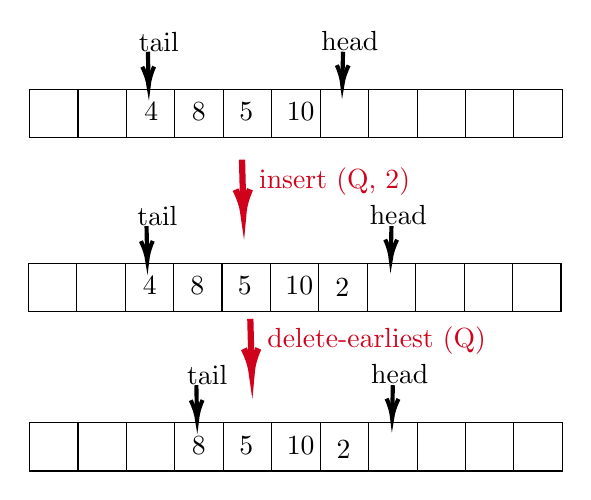
\begin{tikzpicture}[x=0.5pt,y=0.5pt,yscale=-1,xscale=1]
%uncomment if require: \path (0,337); %set diagram left start at 0, and has height of 337

%Shape: Grid [id:dp4942254527972789] 
\draw  [draw opacity=0] (11,49) -- (396,49) -- (396,84) -- (11,84) -- cycle ; \draw   (46,49) -- (46,84)(81,49) -- (81,84)(116,49) -- (116,84)(151,49) -- (151,84)(186,49) -- (186,84)(221,49) -- (221,84)(256,49) -- (256,84)(291,49) -- (291,84)(326,49) -- (326,84)(361,49) -- (361,84) ; \draw    ; \draw   (11,49) -- (396,49) -- (396,84) -- (11,84) -- cycle ;
%Straight Lines [id:da011203202476256058] 
\draw [line width=1.5]    (96.5,22) -- (96.94,44) ;
\draw [shift={(97,47)}, rotate = 268.85] [color={rgb, 255:red, 0; green, 0; blue, 0 }  ][line width=1.5]    (14.21,-4.28) .. controls (9.04,-1.82) and (4.3,-0.39) .. (0,0) .. controls (4.3,0.39) and (9.04,1.82) .. (14.21,4.28)   ;
%Straight Lines [id:da9859159949652865] 
\draw [line width=1.5]    (237.5,22) -- (237.06,43) ;
\draw [shift={(237,46)}, rotate = 271.19] [color={rgb, 255:red, 0; green, 0; blue, 0 }  ][line width=1.5]    (14.21,-4.28) .. controls (9.04,-1.82) and (4.3,-0.39) .. (0,0) .. controls (4.3,0.39) and (9.04,1.82) .. (14.21,4.28)   ;
%Shape: Grid [id:dp8078577975258915] 
\draw  [draw opacity=0] (10,175) -- (395,175) -- (395,210) -- (10,210) -- cycle ; \draw   (45,175) -- (45,210)(80,175) -- (80,210)(115,175) -- (115,210)(150,175) -- (150,210)(185,175) -- (185,210)(220,175) -- (220,210)(255,175) -- (255,210)(290,175) -- (290,210)(325,175) -- (325,210)(360,175) -- (360,210) ; \draw    ; \draw   (10,175) -- (395,175) -- (395,210) -- (10,210) -- cycle ;
%Straight Lines [id:da10073653551255601] 
\draw [line width=1.5]    (95.5,148) -- (95.94,170) ;
\draw [shift={(96,173)}, rotate = 268.85] [color={rgb, 255:red, 0; green, 0; blue, 0 }  ][line width=1.5]    (14.21,-4.28) .. controls (9.04,-1.82) and (4.3,-0.39) .. (0,0) .. controls (4.3,0.39) and (9.04,1.82) .. (14.21,4.28)   ;
%Straight Lines [id:da38679209155686467] 
\draw [line width=1.5]    (272.5,148) -- (272.06,169) ;
\draw [shift={(272,172)}, rotate = 271.19] [color={rgb, 255:red, 0; green, 0; blue, 0 }  ][line width=1.5]    (14.21,-4.28) .. controls (9.04,-1.82) and (4.3,-0.39) .. (0,0) .. controls (4.3,0.39) and (9.04,1.82) .. (14.21,4.28)   ;
%Shape: Grid [id:dp8559849663357562] 
\draw  [draw opacity=0] (11,290) -- (396,290) -- (396,325) -- (11,325) -- cycle ; \draw   (46,290) -- (46,325)(81,290) -- (81,325)(116,290) -- (116,325)(151,290) -- (151,325)(186,290) -- (186,325)(221,290) -- (221,325)(256,290) -- (256,325)(291,290) -- (291,325)(326,290) -- (326,325)(361,290) -- (361,325) ; \draw    ; \draw   (11,290) -- (396,290) -- (396,325) -- (11,325) -- cycle ;
%Straight Lines [id:da6868992534526999] 
\draw [line width=1.5]    (131.5,263) -- (131.94,285) ;
\draw [shift={(132,288)}, rotate = 268.85] [color={rgb, 255:red, 0; green, 0; blue, 0 }  ][line width=1.5]    (14.21,-4.28) .. controls (9.04,-1.82) and (4.3,-0.39) .. (0,0) .. controls (4.3,0.39) and (9.04,1.82) .. (14.21,4.28)   ;
%Straight Lines [id:da16952414255259152] 
\draw [line width=1.5]    (273.5,263) -- (273.06,284) ;
\draw [shift={(273,287)}, rotate = 271.19] [color={rgb, 255:red, 0; green, 0; blue, 0 }  ][line width=1.5]    (14.21,-4.28) .. controls (9.04,-1.82) and (4.3,-0.39) .. (0,0) .. controls (4.3,0.39) and (9.04,1.82) .. (14.21,4.28)   ;
%Straight Lines [id:da21618036120919215] 
\draw [color={rgb, 255:red, 208; green, 2; blue, 27 }  ,draw opacity=1 ][line width=2.25]    (164.5,100) -- (165.4,135) ;
\draw [shift={(165.5,139)}, rotate = 268.53] [color={rgb, 255:red, 208; green, 2; blue, 27 }  ,draw opacity=1 ][line width=2.25]    (17.49,-5.26) .. controls (11.12,-2.23) and (5.29,-0.48) .. (0,0) .. controls (5.29,0.48) and (11.12,2.23) .. (17.49,5.26)   ;
%Straight Lines [id:da7278943927425445] 
\draw [color={rgb, 255:red, 208; green, 2; blue, 27 }  ,draw opacity=1 ][line width=2.25]    (170.5,215) -- (171.4,250) ;
\draw [shift={(171.5,254)}, rotate = 268.53] [color={rgb, 255:red, 208; green, 2; blue, 27 }  ,draw opacity=1 ][line width=2.25]    (17.49,-5.26) .. controls (11.12,-2.23) and (5.29,-0.48) .. (0,0) .. controls (5.29,0.48) and (11.12,2.23) .. (17.49,5.26)   ;

% Text Node
\draw (88,6) node [anchor=north west][inner sep=0.75pt]   [align=left] {tail};
% Text Node
\draw (220,5) node [anchor=north west][inner sep=0.75pt]   [align=left] {head};
% Text Node
\draw (92,57) node [anchor=north west][inner sep=0.75pt]   [align=left] {$\displaystyle 4$};
% Text Node
\draw (126.33,57) node [anchor=north west][inner sep=0.75pt]   [align=left] {$\displaystyle 8$};
% Text Node
\draw (160.66,57) node [anchor=north west][inner sep=0.75pt]   [align=left] {$\displaystyle 5$};
% Text Node
\draw (195,57) node [anchor=north west][inner sep=0.75pt]   [align=left] {$\displaystyle 10$};
% Text Node
\draw (87,132) node [anchor=north west][inner sep=0.75pt]   [align=left] {tail};
% Text Node
\draw (255,131) node [anchor=north west][inner sep=0.75pt]   [align=left] {head};
% Text Node
\draw (91,183) node [anchor=north west][inner sep=0.75pt]   [align=left] {$\displaystyle 4$};
% Text Node
\draw (125.33,183) node [anchor=north west][inner sep=0.75pt]   [align=left] {$\displaystyle 8$};
% Text Node
\draw (159.66,183) node [anchor=north west][inner sep=0.75pt]   [align=left] {$\displaystyle 5$};
% Text Node
\draw (194,183) node [anchor=north west][inner sep=0.75pt]   [align=left] {$\displaystyle 10$};
% Text Node
\draw (123,247) node [anchor=north west][inner sep=0.75pt]   [align=left] {tail};
% Text Node
\draw (256,246) node [anchor=north west][inner sep=0.75pt]   [align=left] {head};
% Text Node
\draw (126.33,298) node [anchor=north west][inner sep=0.75pt]   [align=left] {$\displaystyle 8$};
% Text Node
\draw (160.66,298) node [anchor=north west][inner sep=0.75pt]   [align=left] {$\displaystyle 5$};
% Text Node
\draw (195,298) node [anchor=north west][inner sep=0.75pt]   [align=left] {$\displaystyle 10$};
% Text Node
\draw (175,104) node [anchor=north west][inner sep=0.75pt]   [align=left] {\textcolor[rgb]{0.82,0.01,0.11}{insert (Q, 2)}};
% Text Node
\draw (230,184) node [anchor=north west][inner sep=0.75pt]   [align=left] {$\displaystyle 2$};
% Text Node
\draw (181,219) node [anchor=north west][inner sep=0.75pt]   [align=left] {\textcolor[rgb]{0.82,0.01,0.11}{delete-earliest (Q)}};
% Text Node
\draw (231,301) node [anchor=north west][inner sep=0.75pt]   [align=left] {$\displaystyle 2$};


\end{tikzpicture}

}
\caption{An example of queue.}
\end{figure}

\begin{minipage}{0.8\textwidth}
	\aaA {3}{function empty($Q$)}\xxx
	\aab {if \emph{head} = \emph{tail}: return true;}\xxx
	\aab {else: return false;}\xxx
	\aaa {end function;}\xxx
\end{minipage}

\begin{minipage}{0.8\textwidth}
	\aaA {3}{function insert($Q$, $x$)}\xxx
	\aab {$S[head] = x$;}\xxx
	\aab {head = head + 1;}\xxx
	\aaa {end function;}\xxx
\end{minipage}

\begin{minipage}{0.8\textwidth}
	\aaA {2}{function find-earliest($Q$)}\xxx
	\aab {return $S[tail]$;}\xxx
	\aaa {end function;}\xxx
\end{minipage}

\begin{minipage}{0.8\textwidth}
	\aaA {2}{function delete-earliest($Q$)}\xxx
	\aab {tail = tail + 1;}\xxx
	\aaa {end function;}\xxx
\end{minipage}

Note, a queue data structure exhibits a first-in-first-out property~(while a stack is first-in-last-out).

\section*{Priority Queue}

In a priority queue, each element is associated with a \emph{priority}~(also called key).
In other words, each element in a priority queue is a pair (\emph{key, value}),
where \emph{key} indicates its priority, while \emph{value} stores the actual data.
A \emph{priority queue} data structure supports the following operations.
\vspace*{-\topsep}
\begin{enumerate}
\item empty~($PQ$): decides if priority queue $PQ$ is empty;
\item insert~($PQ$, $x$): add element $x$ to $PQ$;
\item find-min~($PQ$): return the element in $PQ$ with smallest key~(i.e., highest priority);
\item delete-min~($PQ$): remove the element in $PQ$ with smallest key~(i.e., highest priority).
\item decrease-key~($PQ$, pointer-to-an-element, new-key): set the key of the specified element as the given new-key.
\end{enumerate}

Note that a queue can be regarded as a special case of priority, for which the priority
is the time an element is added to the queue.

There are numerous different implementations for priority queue~(check wikipedia). 
Here we introduce one of them, \emph{binary heap}. To do it, let's first
formally introduce \emph{heap}.

%%A \emph{tree} is a connected undirected graph without cycle. A tree with $n$ vertices has $(n - 1)$ edges.
%%A tree can be \emph{rooted} by picking a vertex as root.
%%Such \emph{rooting} procedure adds a direction to each edge~(goes from root to leaves).
%%
%%\begin{figure}[h!]
%%\centering{\tikzset{every picture/.style={line width=0.75pt}} %set default line width to 0.75pt        

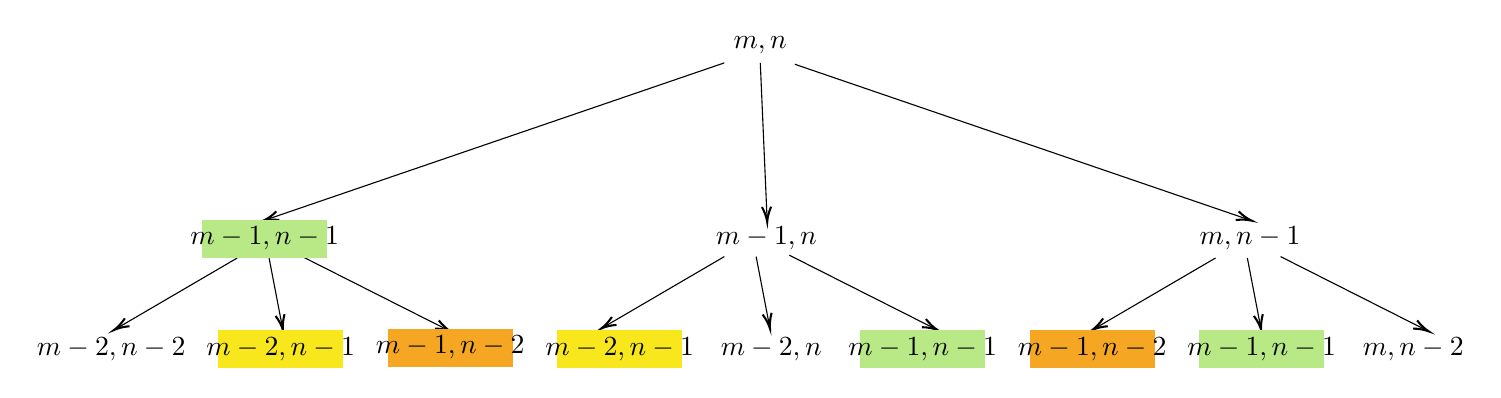
\begin{tikzpicture}[x=0.5pt,y=0.5pt,yscale=-1,xscale=1]
%uncomment if require: \path (0,284); %set diagram left start at 0, and has height of 284

%Straight Lines [id:da1383331413383435] 
\draw    (522.5,36) -- (191.39,149.35) ;
\draw [shift={(189.5,150)}, rotate = 341.1] [color={rgb, 255:red, 0; green, 0; blue, 0 }  ][line width=0.75]    (10.93,-3.29) .. controls (6.95,-1.4) and (3.31,-0.3) .. (0,0) .. controls (3.31,0.3) and (6.95,1.4) .. (10.93,3.29)   ;
%Straight Lines [id:da715204982720897] 
\draw    (548.5,36) -- (553.41,149) ;
\draw [shift={(553.5,151)}, rotate = 267.51] [color={rgb, 255:red, 0; green, 0; blue, 0 }  ][line width=0.75]    (10.93,-3.29) .. controls (6.95,-1.4) and (3.31,-0.3) .. (0,0) .. controls (3.31,0.3) and (6.95,1.4) .. (10.93,3.29)   ;
%Straight Lines [id:da8831806389031782] 
\draw    (573.5,37) -- (901.61,149.35) ;
\draw [shift={(903.5,150)}, rotate = 198.9] [color={rgb, 255:red, 0; green, 0; blue, 0 }  ][line width=0.75]    (10.93,-3.29) .. controls (6.95,-1.4) and (3.31,-0.3) .. (0,0) .. controls (3.31,0.3) and (6.95,1.4) .. (10.93,3.29)   ;
%Straight Lines [id:da6762777724306107] 
\draw    (170.5,177) -- (83.23,227.99) ;
\draw [shift={(81.5,229)}, rotate = 329.7] [color={rgb, 255:red, 0; green, 0; blue, 0 }  ][line width=0.75]    (10.93,-3.29) .. controls (6.95,-1.4) and (3.31,-0.3) .. (0,0) .. controls (3.31,0.3) and (6.95,1.4) .. (10.93,3.29)   ;
%Straight Lines [id:da9537842571445845] 
\draw    (193.5,177) -- (203.12,227.04) ;
\draw [shift={(203.5,229)}, rotate = 259.11] [color={rgb, 255:red, 0; green, 0; blue, 0 }  ][line width=0.75]    (10.93,-3.29) .. controls (6.95,-1.4) and (3.31,-0.3) .. (0,0) .. controls (3.31,0.3) and (6.95,1.4) .. (10.93,3.29)   ;
%Straight Lines [id:da25240177172893863] 
\draw    (217.5,176) -- (322.71,229.1) ;
\draw [shift={(324.5,230)}, rotate = 206.78] [color={rgb, 255:red, 0; green, 0; blue, 0 }  ][line width=0.75]    (10.93,-3.29) .. controls (6.95,-1.4) and (3.31,-0.3) .. (0,0) .. controls (3.31,0.3) and (6.95,1.4) .. (10.93,3.29)   ;
%Straight Lines [id:da4227912867383341] 
\draw    (522.5,176) -- (435.23,226.99) ;
\draw [shift={(433.5,228)}, rotate = 329.7] [color={rgb, 255:red, 0; green, 0; blue, 0 }  ][line width=0.75]    (10.93,-3.29) .. controls (6.95,-1.4) and (3.31,-0.3) .. (0,0) .. controls (3.31,0.3) and (6.95,1.4) .. (10.93,3.29)   ;
%Straight Lines [id:da490335830545392] 
\draw    (545.5,176) -- (555.12,226.04) ;
\draw [shift={(555.5,228)}, rotate = 259.11] [color={rgb, 255:red, 0; green, 0; blue, 0 }  ][line width=0.75]    (10.93,-3.29) .. controls (6.95,-1.4) and (3.31,-0.3) .. (0,0) .. controls (3.31,0.3) and (6.95,1.4) .. (10.93,3.29)   ;
%Straight Lines [id:da44453803269503656] 
\draw    (569.5,175) -- (674.71,228.1) ;
\draw [shift={(676.5,229)}, rotate = 206.78] [color={rgb, 255:red, 0; green, 0; blue, 0 }  ][line width=0.75]    (10.93,-3.29) .. controls (6.95,-1.4) and (3.31,-0.3) .. (0,0) .. controls (3.31,0.3) and (6.95,1.4) .. (10.93,3.29)   ;
%Straight Lines [id:da6159232694423369] 
\draw    (877.5,177) -- (790.23,227.99) ;
\draw [shift={(788.5,229)}, rotate = 329.7] [color={rgb, 255:red, 0; green, 0; blue, 0 }  ][line width=0.75]    (10.93,-3.29) .. controls (6.95,-1.4) and (3.31,-0.3) .. (0,0) .. controls (3.31,0.3) and (6.95,1.4) .. (10.93,3.29)   ;
%Straight Lines [id:da04820263440719896] 
\draw    (900.5,177) -- (910.12,227.04) ;
\draw [shift={(910.5,229)}, rotate = 259.11] [color={rgb, 255:red, 0; green, 0; blue, 0 }  ][line width=0.75]    (10.93,-3.29) .. controls (6.95,-1.4) and (3.31,-0.3) .. (0,0) .. controls (3.31,0.3) and (6.95,1.4) .. (10.93,3.29)   ;
%Straight Lines [id:da4987937509957987] 
\draw    (924.5,176) -- (1029.71,229.1) ;
\draw [shift={(1031.5,230)}, rotate = 206.78] [color={rgb, 255:red, 0; green, 0; blue, 0 }  ][line width=0.75]    (10.93,-3.29) .. controls (6.95,-1.4) and (3.31,-0.3) .. (0,0) .. controls (3.31,0.3) and (6.95,1.4) .. (10.93,3.29)   ;

% Text Node
\draw (548.38,23.47) node   [align=left] {$\displaystyle m,n$};
% Text Node
\draw  [color={rgb, 255:red, 184; green, 233; blue, 134 }  ,draw opacity=1 ][fill={rgb, 255:red, 184; green, 233; blue, 134 }  ,fill opacity=1 ][line width=0.75]   (145.88,149.97) -- (234.88,149.97) -- (234.88,175.97) -- (145.88,175.97) -- cycle  ;
\draw (190.38,162.97) node   [align=left] {$\displaystyle m-1,n-1$};
% Text Node
\draw (552.88,162.97) node   [align=left] {$\displaystyle m-1,n$};
% Text Node
\draw (902.38,162.97) node   [align=left] {$\displaystyle m,n-1$};
% Text Node
\draw (79.38,242.72) node   [align=left] {$\displaystyle m-2,n-2$};
% Text Node
\draw  [color={rgb, 255:red, 248; green, 231; blue, 28 }  ,draw opacity=1 ][fill={rgb, 255:red, 248; green, 231; blue, 28 }  ,fill opacity=1 ][line width=0.75]   (157.38,229.72) -- (246.38,229.72) -- (246.38,255.72) -- (157.38,255.72) -- cycle  ;
\draw (201.88,242.72) node   [align=left] {$\displaystyle m-2,n-1$};
% Text Node
\draw  [color={rgb, 255:red, 245; green, 166; blue, 35 }  ,draw opacity=1 ][fill={rgb, 255:red, 245; green, 166; blue, 35 }  ,fill opacity=1 ][line width=0.75]   (279.88,228.72) -- (368.88,228.72) -- (368.88,254.72) -- (279.88,254.72) -- cycle  ;
\draw (324.38,241.72) node   [align=left] {$\displaystyle m-1,n-2$};
% Text Node
\draw  [color={rgb, 255:red, 248; green, 231; blue, 28 }  ,draw opacity=1 ][fill={rgb, 255:red, 248; green, 231; blue, 28 }  ,fill opacity=1 ][line width=0.75]   (402.38,229.72) -- (491.38,229.72) -- (491.38,255.72) -- (402.38,255.72) -- cycle  ;
\draw (446.88,242.72) node   [align=left] {$\displaystyle m-2,n-1$};
% Text Node
\draw (556.38,242.72) node   [align=left] {$\displaystyle m-2,n$};
% Text Node
\draw  [color={rgb, 255:red, 184; green, 233; blue, 134 }  ,draw opacity=1 ][fill={rgb, 255:red, 184; green, 233; blue, 134 }  ,fill opacity=1 ][line width=0.75]   (621.38,229.72) -- (710.38,229.72) -- (710.38,255.72) -- (621.38,255.72) -- cycle  ;
\draw (665.88,242.72) node   [align=left] {$\displaystyle m-1,n-1$};
% Text Node
\draw  [color={rgb, 255:red, 245; green, 166; blue, 35 }  ,draw opacity=1 ][fill={rgb, 255:red, 245; green, 166; blue, 35 }  ,fill opacity=1 ][line width=0.75]   (743.88,229.72) -- (832.88,229.72) -- (832.88,255.72) -- (743.88,255.72) -- cycle  ;
\draw (788.38,242.72) node   [align=left] {$\displaystyle m-1,n-2$};
% Text Node
\draw  [color={rgb, 255:red, 184; green, 233; blue, 134 }  ,draw opacity=1 ][fill={rgb, 255:red, 184; green, 233; blue, 134 }  ,fill opacity=1 ][line width=0.75]   (866.38,229.72) -- (955.38,229.72) -- (955.38,255.72) -- (866.38,255.72) -- cycle  ;
\draw (910.88,242.72) node   [align=left] {$\displaystyle m-1,n-1$};
% Text Node
\draw (1020.38,242.72) node   [align=left] {$\displaystyle m,n-2$};


\end{tikzpicture}

}
%%\caption{An example of tree and rooting by picking $v_9$ as root.}
%%\end{figure}

A \emph{heap} is a (rooted) tree data structure satisfies the \emph{heap property}.
A heap is either a \emph{min-heap} if it satisfies the \emph{min-heap property}: for any edge $(u, v)$ in the (rooted) tree $T$,
the key of $u$ is smaller than that of $v$,
or a \emph{max-heap} if it satisfies the \emph{max-heap property}: for any edge $(u, v)$ in the (rooted) tree $T$,
the key of $u$ is larger than that of $v$.
Here we always consider a heap as a min-heap, unless otherwise specified.

\begin{figure}[h!]
\centering{

\tikzset{every picture/.style={line width=0.75pt}} %set default line width to 0.75pt        

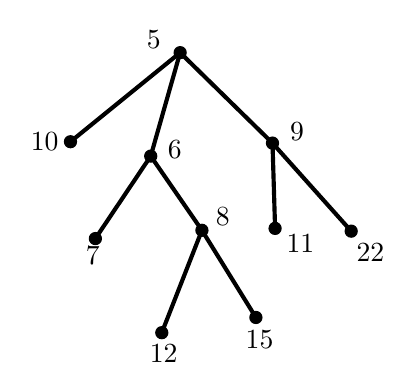
\begin{tikzpicture}[x=0.5pt,y=0.5pt,yscale=-1,xscale=1]
%uncomment if require: \path (0,268); %set diagram left start at 0, and has height of 268

%Flowchart: Connector [id:dp07358279371728427] 
\draw  [fill={rgb, 255:red, 0; green, 0; blue, 0 }  ,fill opacity=1 ] (122.38,22) .. controls (122.38,19.58) and (124.34,17.62) .. (126.75,17.62) .. controls (129.17,17.62) and (131.13,19.58) .. (131.13,22) .. controls (131.13,24.42) and (129.17,26.38) .. (126.75,26.38) .. controls (124.34,26.38) and (122.38,24.42) .. (122.38,22) -- cycle ;
%Flowchart: Connector [id:dp9013708586598245] 
\draw  [fill={rgb, 255:red, 0; green, 0; blue, 0 }  ,fill opacity=1 ] (43.12,86.38) .. controls (43.12,83.96) and (45.08,82) .. (47.5,82) .. controls (49.92,82) and (51.88,83.96) .. (51.88,86.38) .. controls (51.88,88.79) and (49.92,90.75) .. (47.5,90.75) .. controls (45.08,90.75) and (43.12,88.79) .. (43.12,86.38) -- cycle ;
%Flowchart: Connector [id:dp29553697353599095] 
\draw  [fill={rgb, 255:red, 0; green, 0; blue, 0 }  ,fill opacity=1 ] (246,151) .. controls (246,148.58) and (247.96,146.62) .. (250.38,146.62) .. controls (252.79,146.62) and (254.75,148.58) .. (254.75,151) .. controls (254.75,153.42) and (252.79,155.38) .. (250.38,155.38) .. controls (247.96,155.38) and (246,153.42) .. (246,151) -- cycle ;
%Straight Lines [id:da2622599551377074] 
\draw [color={rgb, 255:red, 0; green, 0; blue, 0 }  ,draw opacity=1 ][line width=1.5]    (195.38,149) -- (193.5,87.38) ;
%Straight Lines [id:da633932922371613] 
\draw [color={rgb, 255:red, 0; green, 0; blue, 0 }  ,draw opacity=1 ][line width=1.5]    (47.5,86.38) -- (126.75,22) ;
%Flowchart: Connector [id:dp6006241534205703] 
\draw  [fill={rgb, 255:red, 0; green, 0; blue, 0 }  ,fill opacity=1 ] (101.12,96.75) .. controls (101.12,94.34) and (103.08,92.38) .. (105.5,92.38) .. controls (107.92,92.38) and (109.88,94.34) .. (109.88,96.75) .. controls (109.88,99.17) and (107.92,101.13) .. (105.5,101.13) .. controls (103.08,101.13) and (101.12,99.17) .. (101.12,96.75) -- cycle ;
%Flowchart: Connector [id:dp13162082051454493] 
\draw  [fill={rgb, 255:red, 0; green, 0; blue, 0 }  ,fill opacity=1 ] (189.12,87.38) .. controls (189.12,84.96) and (191.08,83) .. (193.5,83) .. controls (195.92,83) and (197.88,84.96) .. (197.88,87.38) .. controls (197.88,89.79) and (195.92,91.75) .. (193.5,91.75) .. controls (191.08,91.75) and (189.12,89.79) .. (189.12,87.38) -- cycle ;
%Flowchart: Connector [id:dp7155524303373791] 
\draw  [fill={rgb, 255:red, 0; green, 0; blue, 0 }  ,fill opacity=1 ] (61.12,156.38) .. controls (61.12,153.96) and (63.08,152) .. (65.5,152) .. controls (67.92,152) and (69.88,153.96) .. (69.88,156.38) .. controls (69.88,158.79) and (67.92,160.75) .. (65.5,160.75) .. controls (63.08,160.75) and (61.12,158.79) .. (61.12,156.38) -- cycle ;
%Flowchart: Connector [id:dp5160360494307613] 
\draw  [fill={rgb, 255:red, 0; green, 0; blue, 0 }  ,fill opacity=1 ] (138.12,150.38) .. controls (138.12,147.96) and (140.08,146) .. (142.5,146) .. controls (144.92,146) and (146.88,147.96) .. (146.88,150.38) .. controls (146.88,152.79) and (144.92,154.75) .. (142.5,154.75) .. controls (140.08,154.75) and (138.12,152.79) .. (138.12,150.38) -- cycle ;
%Flowchart: Connector [id:dp48925704975832796] 
\draw  [fill={rgb, 255:red, 0; green, 0; blue, 0 }  ,fill opacity=1 ] (109.12,224.38) .. controls (109.12,221.96) and (111.08,220) .. (113.5,220) .. controls (115.92,220) and (117.88,221.96) .. (117.88,224.38) .. controls (117.88,226.79) and (115.92,228.75) .. (113.5,228.75) .. controls (111.08,228.75) and (109.12,226.79) .. (109.12,224.38) -- cycle ;
%Flowchart: Connector [id:dp46343000023437764] 
\draw  [fill={rgb, 255:red, 0; green, 0; blue, 0 }  ,fill opacity=1 ] (177.12,213.38) .. controls (177.12,210.96) and (179.08,209) .. (181.5,209) .. controls (183.92,209) and (185.88,210.96) .. (185.88,213.38) .. controls (185.88,215.79) and (183.92,217.75) .. (181.5,217.75) .. controls (179.08,217.75) and (177.12,215.79) .. (177.12,213.38) -- cycle ;
%Straight Lines [id:da8627932820811317] 
\draw [color={rgb, 255:red, 0; green, 0; blue, 0 }  ,draw opacity=1 ][line width=1.5]    (105.5,96.75) -- (126.75,22) ;
%Straight Lines [id:da5409521442924461] 
\draw [color={rgb, 255:red, 0; green, 0; blue, 0 }  ,draw opacity=1 ][line width=1.5]    (193.5,87.38) -- (126.75,22) ;
%Straight Lines [id:da6747902580631686] 
\draw [color={rgb, 255:red, 0; green, 0; blue, 0 }  ,draw opacity=1 ][line width=1.5]    (65.5,156.38) -- (105.5,96.75) ;
%Straight Lines [id:da9660976210409085] 
\draw [color={rgb, 255:red, 0; green, 0; blue, 0 }  ,draw opacity=1 ][line width=1.5]    (142.5,150.38) -- (105.5,96.75) ;
%Straight Lines [id:da7815420677213977] 
\draw [color={rgb, 255:red, 0; green, 0; blue, 0 }  ,draw opacity=1 ][line width=1.5]    (113.5,224.38) -- (142.5,150.38) ;
%Straight Lines [id:da6594188595232979] 
\draw [color={rgb, 255:red, 0; green, 0; blue, 0 }  ,draw opacity=1 ][line width=1.5]    (181.5,213.38) -- (142.5,150.38) ;
%Flowchart: Connector [id:dp9035939512481367] 
\draw  [fill={rgb, 255:red, 0; green, 0; blue, 0 }  ,fill opacity=1 ] (191,149) .. controls (191,146.58) and (192.96,144.62) .. (195.38,144.62) .. controls (197.79,144.62) and (199.75,146.58) .. (199.75,149) .. controls (199.75,151.42) and (197.79,153.38) .. (195.38,153.38) .. controls (192.96,153.38) and (191,151.42) .. (191,149) -- cycle ;
%Straight Lines [id:da9909770061710292] 
\draw [color={rgb, 255:red, 0; green, 0; blue, 0 }  ,draw opacity=1 ][line width=1.5]    (250.38,151) -- (193.5,87.38) ;

% Text Node
\draw (116,84) node [anchor=north west][inner sep=0.75pt]   [align=left] {$\displaystyle 6$};
% Text Node
\draw (172.24,221.06) node [anchor=north west][inner sep=0.75pt]   [align=left] {$\displaystyle 15$};
% Text Node
\draw (56.75,160) node [anchor=north west][inner sep=0.75pt]   [align=left] {$\displaystyle 7$};
% Text Node
\draw (204.38,70.38) node [anchor=north west][inner sep=0.75pt]   [align=left] {$\displaystyle 9$};
% Text Node
\draw (252.38,158.38) node [anchor=north west][inner sep=0.75pt]   [align=left] {$\displaystyle 22$};
% Text Node
\draw (201.75,152) node [anchor=north west][inner sep=0.75pt]   [align=left] {$\displaystyle 11$};
% Text Node
\draw (150.75,132.35) node [anchor=north west][inner sep=0.75pt]   [align=left] {$\displaystyle 8$};
% Text Node
\draw (102.97,230.91) node [anchor=north west][inner sep=0.75pt]   [align=left] {$\displaystyle 12$};
% Text Node
\draw (16.97,77.91) node [anchor=north west][inner sep=0.75pt]   [align=left] {$\displaystyle 10$};
% Text Node
\draw (100.75,4.35) node [anchor=north west][inner sep=0.75pt]   [align=left] {$\displaystyle 5$};


\end{tikzpicture}

}
\caption{An example of heap. The key of an element is next to vertices}
\end{figure}

A \emph{binary heap} is a heap with the tree being the \emph{complete binary tree}.
A \emph{complete binary tree} is a binary tree~(i.e., each vertex has at most 2 children)
and that in every layer of the tree, except possibly the last, is completely filled, and all vertices in the last layer are placed from left to right.

\begin{figure}[h!]
\centering{

\tikzset{every picture/.style={line width=0.75pt}} %set default line width to 0.75pt        

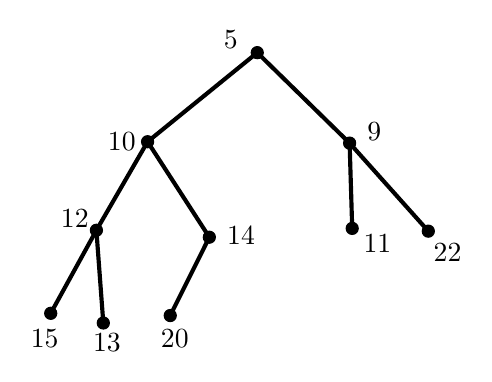
\begin{tikzpicture}[x=0.5pt,y=0.5pt,yscale=-1,xscale=1]
%uncomment if require: \path (0,253); %set diagram left start at 0, and has height of 253

%Flowchart: Connector [id:dp07358279371728427] 
\draw  [fill={rgb, 255:red, 0; green, 0; blue, 0 }  ,fill opacity=1 ] (176.38,22) .. controls (176.38,19.58) and (178.34,17.62) .. (180.75,17.62) .. controls (183.17,17.62) and (185.13,19.58) .. (185.13,22) .. controls (185.13,24.42) and (183.17,26.38) .. (180.75,26.38) .. controls (178.34,26.38) and (176.38,24.42) .. (176.38,22) -- cycle ;
%Flowchart: Connector [id:dp9013708586598245] 
\draw  [fill={rgb, 255:red, 0; green, 0; blue, 0 }  ,fill opacity=1 ] (97.12,86.38) .. controls (97.12,83.96) and (99.08,82) .. (101.5,82) .. controls (103.92,82) and (105.88,83.96) .. (105.88,86.38) .. controls (105.88,88.79) and (103.92,90.75) .. (101.5,90.75) .. controls (99.08,90.75) and (97.12,88.79) .. (97.12,86.38) -- cycle ;
%Flowchart: Connector [id:dp29553697353599095] 
\draw  [fill={rgb, 255:red, 0; green, 0; blue, 0 }  ,fill opacity=1 ] (300,151) .. controls (300,148.58) and (301.96,146.62) .. (304.38,146.62) .. controls (306.79,146.62) and (308.75,148.58) .. (308.75,151) .. controls (308.75,153.42) and (306.79,155.38) .. (304.38,155.38) .. controls (301.96,155.38) and (300,153.42) .. (300,151) -- cycle ;
%Straight Lines [id:da2622599551377074] 
\draw [color={rgb, 255:red, 0; green, 0; blue, 0 }  ,draw opacity=1 ][line width=1.5]    (249.38,149) -- (247.5,87.38) ;
%Straight Lines [id:da633932922371613] 
\draw [color={rgb, 255:red, 0; green, 0; blue, 0 }  ,draw opacity=1 ][line width=1.5]    (101.5,86.38) -- (180.75,22) ;
%Flowchart: Connector [id:dp13162082051454493] 
\draw  [fill={rgb, 255:red, 0; green, 0; blue, 0 }  ,fill opacity=1 ] (243.12,87.38) .. controls (243.12,84.96) and (245.08,83) .. (247.5,83) .. controls (249.92,83) and (251.88,84.96) .. (251.88,87.38) .. controls (251.88,89.79) and (249.92,91.75) .. (247.5,91.75) .. controls (245.08,91.75) and (243.12,89.79) .. (243.12,87.38) -- cycle ;
%Flowchart: Connector [id:dp7155524303373791] 
\draw  [fill={rgb, 255:red, 0; green, 0; blue, 0 }  ,fill opacity=1 ] (60.12,150.38) .. controls (60.12,147.96) and (62.08,146) .. (64.5,146) .. controls (66.92,146) and (68.88,147.96) .. (68.88,150.38) .. controls (68.88,152.79) and (66.92,154.75) .. (64.5,154.75) .. controls (62.08,154.75) and (60.12,152.79) .. (60.12,150.38) -- cycle ;
%Flowchart: Connector [id:dp46343000023437764] 
\draw  [fill={rgb, 255:red, 0; green, 0; blue, 0 }  ,fill opacity=1 ] (27.12,210.38) .. controls (27.12,207.96) and (29.08,206) .. (31.5,206) .. controls (33.92,206) and (35.88,207.96) .. (35.88,210.38) .. controls (35.88,212.79) and (33.92,214.75) .. (31.5,214.75) .. controls (29.08,214.75) and (27.12,212.79) .. (27.12,210.38) -- cycle ;
%Straight Lines [id:da5409521442924461] 
\draw [color={rgb, 255:red, 0; green, 0; blue, 0 }  ,draw opacity=1 ][line width=1.5]    (247.5,87.38) -- (180.75,22) ;
%Straight Lines [id:da6747902580631686] 
\draw [color={rgb, 255:red, 0; green, 0; blue, 0 }  ,draw opacity=1 ][line width=1.5]    (64.5,150.38) -- (101.5,86.38) ;
%Straight Lines [id:da7815420677213977] 
\draw [color={rgb, 255:red, 0; green, 0; blue, 0 }  ,draw opacity=1 ][line width=1.5]    (146.12,155.38) -- (101.5,86.38) ;
%Straight Lines [id:da6594188595232979] 
\draw [color={rgb, 255:red, 0; green, 0; blue, 0 }  ,draw opacity=1 ][line width=1.5]    (31.5,210.38) -- (64.5,150.38) ;
%Flowchart: Connector [id:dp9035939512481367] 
\draw  [fill={rgb, 255:red, 0; green, 0; blue, 0 }  ,fill opacity=1 ] (245,149) .. controls (245,146.58) and (246.96,144.62) .. (249.38,144.62) .. controls (251.79,144.62) and (253.75,146.58) .. (253.75,149) .. controls (253.75,151.42) and (251.79,153.38) .. (249.38,153.38) .. controls (246.96,153.38) and (245,151.42) .. (245,149) -- cycle ;
%Straight Lines [id:da9909770061710292] 
\draw [color={rgb, 255:red, 0; green, 0; blue, 0 }  ,draw opacity=1 ][line width=1.5]    (304.38,151) -- (247.5,87.38) ;
%Flowchart: Connector [id:dp5892893328284525] 
\draw  [fill={rgb, 255:red, 0; green, 0; blue, 0 }  ,fill opacity=1 ] (65.12,217.38) .. controls (65.12,214.96) and (67.08,213) .. (69.5,213) .. controls (71.92,213) and (73.88,214.96) .. (73.88,217.38) .. controls (73.88,219.79) and (71.92,221.75) .. (69.5,221.75) .. controls (67.08,221.75) and (65.12,219.79) .. (65.12,217.38) -- cycle ;
%Flowchart: Connector [id:dp37796994403666173] 
\draw  [fill={rgb, 255:red, 0; green, 0; blue, 0 }  ,fill opacity=1 ] (113.5,212) .. controls (113.5,209.58) and (115.46,207.62) .. (117.88,207.62) .. controls (120.29,207.62) and (122.25,209.58) .. (122.25,212) .. controls (122.25,214.42) and (120.29,216.38) .. (117.88,216.38) .. controls (115.46,216.38) and (113.5,214.42) .. (113.5,212) -- cycle ;
%Flowchart: Connector [id:dp4981451941949617] 
\draw  [fill={rgb, 255:red, 0; green, 0; blue, 0 }  ,fill opacity=1 ] (141.75,155.38) .. controls (141.75,152.96) and (143.71,151) .. (146.12,151) .. controls (148.54,151) and (150.5,152.96) .. (150.5,155.38) .. controls (150.5,157.79) and (148.54,159.75) .. (146.12,159.75) .. controls (143.71,159.75) and (141.75,157.79) .. (141.75,155.38) -- cycle ;
%Straight Lines [id:da07065002309169843] 
\draw [color={rgb, 255:red, 0; green, 0; blue, 0 }  ,draw opacity=1 ][line width=1.5]    (69.5,217.38) -- (64.5,150.38) ;
%Straight Lines [id:da3423526836996703] 
\draw [color={rgb, 255:red, 0; green, 0; blue, 0 }  ,draw opacity=1 ][line width=1.5]    (117.88,212) -- (146.12,155.38) ;

% Text Node
\draw (15.24,220.06) node [anchor=north west][inner sep=0.75pt]   [align=left] {$\displaystyle 15$};
% Text Node
\draw (258.38,70.38) node [anchor=north west][inner sep=0.75pt]   [align=left] {$\displaystyle 9$};
% Text Node
\draw (306.38,158.38) node [anchor=north west][inner sep=0.75pt]   [align=left] {$\displaystyle 22$};
% Text Node
\draw (255.75,152) node [anchor=north west][inner sep=0.75pt]   [align=left] {$\displaystyle 11$};
% Text Node
\draw (36.97,133.91) node [anchor=north west][inner sep=0.75pt]   [align=left] {$\displaystyle 12$};
% Text Node
\draw (70.97,77.91) node [anchor=north west][inner sep=0.75pt]   [align=left] {$\displaystyle 10$};
% Text Node
\draw (154.75,4.35) node [anchor=north west][inner sep=0.75pt]   [align=left] {$\displaystyle 5$};
% Text Node
\draw (60.24,223.47) node [anchor=north west][inner sep=0.75pt]   [align=left] {$\displaystyle 13$};
% Text Node
\draw (109.25,220) node [anchor=north west][inner sep=0.75pt]   [align=left] {$\displaystyle 20$};
% Text Node
\draw (157.12,145.75) node [anchor=north west][inner sep=0.75pt]   [align=left] {$\displaystyle 14$};


\end{tikzpicture}

}
\caption{An example of binary heap.}
\end{figure}

Since a binary heap $T$ is so regular, we can use an array $S$ to store its elements~(rather than using adjacency list).
The root~(i.e., layer 0) of $T$ is placed in $S[1]$~(we assume that the index of $S$ starts from 1),
the first element of the layer~1 is placed in $S[2]$, and so on.
Generally, the $j$-th element in the $i$-th layer of $T$ will be placed in $S[2^i + j - 1]$.
%Using an array to store a binary heap $T$, 
We can also easily access the parent and children of an element:
\vspace*{-\topsep}
\begin{enumerate}
\item the parent element of $S[k]$ is $S[k/2]$~(floor of $k/2$);
\item the left child of $S[k]$ is $S[2k]$; the right child of $S[k]$ is $S[2k + 1]$.
\end{enumerate}

We now introduce two common procedures used in implementing a binary heap.
These procedures apply when one vertex violates the heap property,
and they can adjust the heap to make it satisfy the heap property.

The \emph{bubble-up} function applies when a vertex has a smaller key than its parent.

\begin{minipage}{0.8\textwidth}
	\aaA {6}{function bubble-up~($S$, $k$)}\xxx
	\aab {$p = k / 2$;}\xxx
	\aaB {3}{if ($S[k].key < S[p].key$);}\xxx
	\aac {swap $S[p]$ and $S[k]$;}\xxx
	\aac {bubble-up~($S$, $p$);}\xxx
	\aab {end if;}\xxx
	\aaa {end function;}\xxx
\end{minipage}

\begin{figure}[h!]
\centering{

\tikzset{every picture/.style={line width=0.75pt}} %set default line width to 0.75pt        

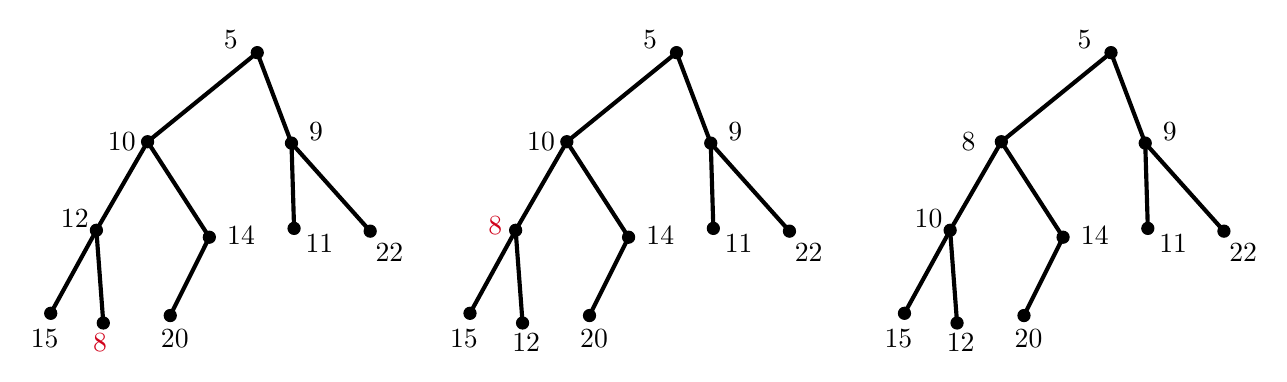
\begin{tikzpicture}[x=0.5pt,y=0.5pt,yscale=-1,xscale=1]
%uncomment if require: \path (0,251); %set diagram left start at 0, and has height of 251

%Flowchart: Connector [id:dp07358279371728427] 
\draw  [fill={rgb, 255:red, 0; green, 0; blue, 0 }  ,fill opacity=1 ] (176.38,20) .. controls (176.38,17.58) and (178.34,15.62) .. (180.75,15.62) .. controls (183.17,15.62) and (185.13,17.58) .. (185.13,20) .. controls (185.13,22.42) and (183.17,24.38) .. (180.75,24.38) .. controls (178.34,24.38) and (176.38,22.42) .. (176.38,20) -- cycle ;
%Flowchart: Connector [id:dp9013708586598245] 
\draw  [fill={rgb, 255:red, 0; green, 0; blue, 0 }  ,fill opacity=1 ] (97.12,84.38) .. controls (97.12,81.96) and (99.08,80) .. (101.5,80) .. controls (103.92,80) and (105.88,81.96) .. (105.88,84.38) .. controls (105.88,86.79) and (103.92,88.75) .. (101.5,88.75) .. controls (99.08,88.75) and (97.12,86.79) .. (97.12,84.38) -- cycle ;
%Flowchart: Connector [id:dp29553697353599095] 
\draw  [fill={rgb, 255:red, 0; green, 0; blue, 0 }  ,fill opacity=1 ] (258,149) .. controls (258,146.58) and (259.96,144.62) .. (262.38,144.62) .. controls (264.79,144.62) and (266.75,146.58) .. (266.75,149) .. controls (266.75,151.42) and (264.79,153.38) .. (262.38,153.38) .. controls (259.96,153.38) and (258,151.42) .. (258,149) -- cycle ;
%Straight Lines [id:da2622599551377074] 
\draw [color={rgb, 255:red, 0; green, 0; blue, 0 }  ,draw opacity=1 ][line width=1.5]    (207.38,147) -- (205.5,85.38) ;
%Straight Lines [id:da633932922371613] 
\draw [color={rgb, 255:red, 0; green, 0; blue, 0 }  ,draw opacity=1 ][line width=1.5]    (101.5,84.38) -- (180.75,20) ;
%Flowchart: Connector [id:dp13162082051454493] 
\draw  [fill={rgb, 255:red, 0; green, 0; blue, 0 }  ,fill opacity=1 ] (201.12,85.38) .. controls (201.12,82.96) and (203.08,81) .. (205.5,81) .. controls (207.92,81) and (209.88,82.96) .. (209.88,85.38) .. controls (209.88,87.79) and (207.92,89.75) .. (205.5,89.75) .. controls (203.08,89.75) and (201.12,87.79) .. (201.12,85.38) -- cycle ;
%Flowchart: Connector [id:dp7155524303373791] 
\draw  [fill={rgb, 255:red, 0; green, 0; blue, 0 }  ,fill opacity=1 ] (60.12,148.38) .. controls (60.12,145.96) and (62.08,144) .. (64.5,144) .. controls (66.92,144) and (68.88,145.96) .. (68.88,148.38) .. controls (68.88,150.79) and (66.92,152.75) .. (64.5,152.75) .. controls (62.08,152.75) and (60.12,150.79) .. (60.12,148.38) -- cycle ;
%Flowchart: Connector [id:dp46343000023437764] 
\draw  [fill={rgb, 255:red, 0; green, 0; blue, 0 }  ,fill opacity=1 ] (27.12,208.38) .. controls (27.12,205.96) and (29.08,204) .. (31.5,204) .. controls (33.92,204) and (35.88,205.96) .. (35.88,208.38) .. controls (35.88,210.79) and (33.92,212.75) .. (31.5,212.75) .. controls (29.08,212.75) and (27.12,210.79) .. (27.12,208.38) -- cycle ;
%Straight Lines [id:da5409521442924461] 
\draw [color={rgb, 255:red, 0; green, 0; blue, 0 }  ,draw opacity=1 ][line width=1.5]    (205.5,85.38) -- (180.75,20) ;
%Straight Lines [id:da6747902580631686] 
\draw [color={rgb, 255:red, 0; green, 0; blue, 0 }  ,draw opacity=1 ][line width=1.5]    (64.5,148.38) -- (101.5,84.38) ;
%Straight Lines [id:da7815420677213977] 
\draw [color={rgb, 255:red, 0; green, 0; blue, 0 }  ,draw opacity=1 ][line width=1.5]    (146.12,153.38) -- (101.5,84.38) ;
%Straight Lines [id:da6594188595232979] 
\draw [color={rgb, 255:red, 0; green, 0; blue, 0 }  ,draw opacity=1 ][line width=1.5]    (31.5,208.38) -- (64.5,148.38) ;
%Flowchart: Connector [id:dp9035939512481367] 
\draw  [fill={rgb, 255:red, 0; green, 0; blue, 0 }  ,fill opacity=1 ] (203,147) .. controls (203,144.58) and (204.96,142.62) .. (207.38,142.62) .. controls (209.79,142.62) and (211.75,144.58) .. (211.75,147) .. controls (211.75,149.42) and (209.79,151.38) .. (207.38,151.38) .. controls (204.96,151.38) and (203,149.42) .. (203,147) -- cycle ;
%Straight Lines [id:da9909770061710292] 
\draw [color={rgb, 255:red, 0; green, 0; blue, 0 }  ,draw opacity=1 ][line width=1.5]    (262.38,149) -- (205.5,85.38) ;
%Flowchart: Connector [id:dp5892893328284525] 
\draw  [fill={rgb, 255:red, 0; green, 0; blue, 0 }  ,fill opacity=1 ] (65.12,215.38) .. controls (65.12,212.96) and (67.08,211) .. (69.5,211) .. controls (71.92,211) and (73.88,212.96) .. (73.88,215.38) .. controls (73.88,217.79) and (71.92,219.75) .. (69.5,219.75) .. controls (67.08,219.75) and (65.12,217.79) .. (65.12,215.38) -- cycle ;
%Flowchart: Connector [id:dp37796994403666173] 
\draw  [fill={rgb, 255:red, 0; green, 0; blue, 0 }  ,fill opacity=1 ] (113.5,210) .. controls (113.5,207.58) and (115.46,205.62) .. (117.88,205.62) .. controls (120.29,205.62) and (122.25,207.58) .. (122.25,210) .. controls (122.25,212.42) and (120.29,214.38) .. (117.88,214.38) .. controls (115.46,214.38) and (113.5,212.42) .. (113.5,210) -- cycle ;
%Flowchart: Connector [id:dp4981451941949617] 
\draw  [fill={rgb, 255:red, 0; green, 0; blue, 0 }  ,fill opacity=1 ] (141.75,153.38) .. controls (141.75,150.96) and (143.71,149) .. (146.12,149) .. controls (148.54,149) and (150.5,150.96) .. (150.5,153.38) .. controls (150.5,155.79) and (148.54,157.75) .. (146.12,157.75) .. controls (143.71,157.75) and (141.75,155.79) .. (141.75,153.38) -- cycle ;
%Straight Lines [id:da07065002309169843] 
\draw [color={rgb, 255:red, 0; green, 0; blue, 0 }  ,draw opacity=1 ][line width=1.5]    (69.5,215.38) -- (64.5,148.38) ;
%Straight Lines [id:da3423526836996703] 
\draw [color={rgb, 255:red, 0; green, 0; blue, 0 }  ,draw opacity=1 ][line width=1.5]    (117.88,210) -- (146.12,153.38) ;
%Flowchart: Connector [id:dp1375963085229701] 
\draw  [fill={rgb, 255:red, 0; green, 0; blue, 0 }  ,fill opacity=1 ] (479.38,20) .. controls (479.38,17.58) and (481.34,15.62) .. (483.75,15.62) .. controls (486.17,15.62) and (488.13,17.58) .. (488.13,20) .. controls (488.13,22.42) and (486.17,24.38) .. (483.75,24.38) .. controls (481.34,24.38) and (479.38,22.42) .. (479.38,20) -- cycle ;
%Flowchart: Connector [id:dp09051194852712707] 
\draw  [fill={rgb, 255:red, 0; green, 0; blue, 0 }  ,fill opacity=1 ] (400.12,84.38) .. controls (400.12,81.96) and (402.08,80) .. (404.5,80) .. controls (406.92,80) and (408.88,81.96) .. (408.88,84.38) .. controls (408.88,86.79) and (406.92,88.75) .. (404.5,88.75) .. controls (402.08,88.75) and (400.12,86.79) .. (400.12,84.38) -- cycle ;
%Flowchart: Connector [id:dp4526533094703221] 
\draw  [fill={rgb, 255:red, 0; green, 0; blue, 0 }  ,fill opacity=1 ] (561,149) .. controls (561,146.58) and (562.96,144.62) .. (565.38,144.62) .. controls (567.79,144.62) and (569.75,146.58) .. (569.75,149) .. controls (569.75,151.42) and (567.79,153.38) .. (565.38,153.38) .. controls (562.96,153.38) and (561,151.42) .. (561,149) -- cycle ;
%Straight Lines [id:da10531615798128313] 
\draw [color={rgb, 255:red, 0; green, 0; blue, 0 }  ,draw opacity=1 ][line width=1.5]    (510.38,147) -- (508.5,85.38) ;
%Straight Lines [id:da09372307643584044] 
\draw [color={rgb, 255:red, 0; green, 0; blue, 0 }  ,draw opacity=1 ][line width=1.5]    (404.5,84.38) -- (483.75,20) ;
%Flowchart: Connector [id:dp8971420943691574] 
\draw  [fill={rgb, 255:red, 0; green, 0; blue, 0 }  ,fill opacity=1 ] (504.12,85.38) .. controls (504.12,82.96) and (506.08,81) .. (508.5,81) .. controls (510.92,81) and (512.88,82.96) .. (512.88,85.38) .. controls (512.88,87.79) and (510.92,89.75) .. (508.5,89.75) .. controls (506.08,89.75) and (504.12,87.79) .. (504.12,85.38) -- cycle ;
%Flowchart: Connector [id:dp12888541856196722] 
\draw  [fill={rgb, 255:red, 0; green, 0; blue, 0 }  ,fill opacity=1 ] (363.12,148.38) .. controls (363.12,145.96) and (365.08,144) .. (367.5,144) .. controls (369.92,144) and (371.88,145.96) .. (371.88,148.38) .. controls (371.88,150.79) and (369.92,152.75) .. (367.5,152.75) .. controls (365.08,152.75) and (363.12,150.79) .. (363.12,148.38) -- cycle ;
%Flowchart: Connector [id:dp37976886359787154] 
\draw  [fill={rgb, 255:red, 0; green, 0; blue, 0 }  ,fill opacity=1 ] (330.12,208.38) .. controls (330.12,205.96) and (332.08,204) .. (334.5,204) .. controls (336.92,204) and (338.88,205.96) .. (338.88,208.38) .. controls (338.88,210.79) and (336.92,212.75) .. (334.5,212.75) .. controls (332.08,212.75) and (330.12,210.79) .. (330.12,208.38) -- cycle ;
%Straight Lines [id:da00382939631379986] 
\draw [color={rgb, 255:red, 0; green, 0; blue, 0 }  ,draw opacity=1 ][line width=1.5]    (508.5,85.38) -- (483.75,20) ;
%Straight Lines [id:da5006261717026612] 
\draw [color={rgb, 255:red, 0; green, 0; blue, 0 }  ,draw opacity=1 ][line width=1.5]    (367.5,148.38) -- (404.5,84.38) ;
%Straight Lines [id:da3231292917624934] 
\draw [color={rgb, 255:red, 0; green, 0; blue, 0 }  ,draw opacity=1 ][line width=1.5]    (449.12,153.38) -- (404.5,84.38) ;
%Straight Lines [id:da6003626275111184] 
\draw [color={rgb, 255:red, 0; green, 0; blue, 0 }  ,draw opacity=1 ][line width=1.5]    (334.5,208.38) -- (367.5,148.38) ;
%Flowchart: Connector [id:dp24928242887719] 
\draw  [fill={rgb, 255:red, 0; green, 0; blue, 0 }  ,fill opacity=1 ] (506,147) .. controls (506,144.58) and (507.96,142.62) .. (510.38,142.62) .. controls (512.79,142.62) and (514.75,144.58) .. (514.75,147) .. controls (514.75,149.42) and (512.79,151.38) .. (510.38,151.38) .. controls (507.96,151.38) and (506,149.42) .. (506,147) -- cycle ;
%Straight Lines [id:da8874329094923221] 
\draw [color={rgb, 255:red, 0; green, 0; blue, 0 }  ,draw opacity=1 ][line width=1.5]    (565.38,149) -- (508.5,85.38) ;
%Flowchart: Connector [id:dp9376179775043852] 
\draw  [fill={rgb, 255:red, 0; green, 0; blue, 0 }  ,fill opacity=1 ] (368.12,215.38) .. controls (368.12,212.96) and (370.08,211) .. (372.5,211) .. controls (374.92,211) and (376.88,212.96) .. (376.88,215.38) .. controls (376.88,217.79) and (374.92,219.75) .. (372.5,219.75) .. controls (370.08,219.75) and (368.12,217.79) .. (368.12,215.38) -- cycle ;
%Flowchart: Connector [id:dp5490426987923039] 
\draw  [fill={rgb, 255:red, 0; green, 0; blue, 0 }  ,fill opacity=1 ] (416.5,210) .. controls (416.5,207.58) and (418.46,205.62) .. (420.88,205.62) .. controls (423.29,205.62) and (425.25,207.58) .. (425.25,210) .. controls (425.25,212.42) and (423.29,214.38) .. (420.88,214.38) .. controls (418.46,214.38) and (416.5,212.42) .. (416.5,210) -- cycle ;
%Flowchart: Connector [id:dp3451316924285829] 
\draw  [fill={rgb, 255:red, 0; green, 0; blue, 0 }  ,fill opacity=1 ] (444.75,153.38) .. controls (444.75,150.96) and (446.71,149) .. (449.12,149) .. controls (451.54,149) and (453.5,150.96) .. (453.5,153.38) .. controls (453.5,155.79) and (451.54,157.75) .. (449.12,157.75) .. controls (446.71,157.75) and (444.75,155.79) .. (444.75,153.38) -- cycle ;
%Straight Lines [id:da35613207019768434] 
\draw [color={rgb, 255:red, 0; green, 0; blue, 0 }  ,draw opacity=1 ][line width=1.5]    (372.5,215.38) -- (367.5,148.38) ;
%Straight Lines [id:da5174013869010234] 
\draw [color={rgb, 255:red, 0; green, 0; blue, 0 }  ,draw opacity=1 ][line width=1.5]    (420.88,210) -- (449.12,153.38) ;
%Flowchart: Connector [id:dp6439356336322] 
\draw  [fill={rgb, 255:red, 0; green, 0; blue, 0 }  ,fill opacity=1 ] (793.38,20) .. controls (793.38,17.58) and (795.34,15.62) .. (797.75,15.62) .. controls (800.17,15.62) and (802.13,17.58) .. (802.13,20) .. controls (802.13,22.42) and (800.17,24.38) .. (797.75,24.38) .. controls (795.34,24.38) and (793.38,22.42) .. (793.38,20) -- cycle ;
%Flowchart: Connector [id:dp21886990424308195] 
\draw  [fill={rgb, 255:red, 0; green, 0; blue, 0 }  ,fill opacity=1 ] (714.12,84.38) .. controls (714.12,81.96) and (716.08,80) .. (718.5,80) .. controls (720.92,80) and (722.88,81.96) .. (722.88,84.38) .. controls (722.88,86.79) and (720.92,88.75) .. (718.5,88.75) .. controls (716.08,88.75) and (714.12,86.79) .. (714.12,84.38) -- cycle ;
%Flowchart: Connector [id:dp03837895619274634] 
\draw  [fill={rgb, 255:red, 0; green, 0; blue, 0 }  ,fill opacity=1 ] (875,149) .. controls (875,146.58) and (876.96,144.62) .. (879.38,144.62) .. controls (881.79,144.62) and (883.75,146.58) .. (883.75,149) .. controls (883.75,151.42) and (881.79,153.38) .. (879.38,153.38) .. controls (876.96,153.38) and (875,151.42) .. (875,149) -- cycle ;
%Straight Lines [id:da14782465407982648] 
\draw [color={rgb, 255:red, 0; green, 0; blue, 0 }  ,draw opacity=1 ][line width=1.5]    (824.38,147) -- (822.5,85.38) ;
%Straight Lines [id:da008115829235638361] 
\draw [color={rgb, 255:red, 0; green, 0; blue, 0 }  ,draw opacity=1 ][line width=1.5]    (718.5,84.38) -- (797.75,20) ;
%Flowchart: Connector [id:dp749580488735119] 
\draw  [fill={rgb, 255:red, 0; green, 0; blue, 0 }  ,fill opacity=1 ] (818.12,85.38) .. controls (818.12,82.96) and (820.08,81) .. (822.5,81) .. controls (824.92,81) and (826.88,82.96) .. (826.88,85.38) .. controls (826.88,87.79) and (824.92,89.75) .. (822.5,89.75) .. controls (820.08,89.75) and (818.12,87.79) .. (818.12,85.38) -- cycle ;
%Flowchart: Connector [id:dp721237398452121] 
\draw  [fill={rgb, 255:red, 0; green, 0; blue, 0 }  ,fill opacity=1 ] (677.12,148.38) .. controls (677.12,145.96) and (679.08,144) .. (681.5,144) .. controls (683.92,144) and (685.88,145.96) .. (685.88,148.38) .. controls (685.88,150.79) and (683.92,152.75) .. (681.5,152.75) .. controls (679.08,152.75) and (677.12,150.79) .. (677.12,148.38) -- cycle ;
%Flowchart: Connector [id:dp8969752490868951] 
\draw  [fill={rgb, 255:red, 0; green, 0; blue, 0 }  ,fill opacity=1 ] (644.12,208.38) .. controls (644.12,205.96) and (646.08,204) .. (648.5,204) .. controls (650.92,204) and (652.88,205.96) .. (652.88,208.38) .. controls (652.88,210.79) and (650.92,212.75) .. (648.5,212.75) .. controls (646.08,212.75) and (644.12,210.79) .. (644.12,208.38) -- cycle ;
%Straight Lines [id:da1950712786856147] 
\draw [color={rgb, 255:red, 0; green, 0; blue, 0 }  ,draw opacity=1 ][line width=1.5]    (822.5,85.38) -- (797.75,20) ;
%Straight Lines [id:da5410491903490715] 
\draw [color={rgb, 255:red, 0; green, 0; blue, 0 }  ,draw opacity=1 ][line width=1.5]    (681.5,148.38) -- (718.5,84.38) ;
%Straight Lines [id:da13743949368590924] 
\draw [color={rgb, 255:red, 0; green, 0; blue, 0 }  ,draw opacity=1 ][line width=1.5]    (763.12,153.38) -- (718.5,84.38) ;
%Straight Lines [id:da3696523456420949] 
\draw [color={rgb, 255:red, 0; green, 0; blue, 0 }  ,draw opacity=1 ][line width=1.5]    (648.5,208.38) -- (681.5,148.38) ;
%Flowchart: Connector [id:dp0084873615551605] 
\draw  [fill={rgb, 255:red, 0; green, 0; blue, 0 }  ,fill opacity=1 ] (820,147) .. controls (820,144.58) and (821.96,142.62) .. (824.38,142.62) .. controls (826.79,142.62) and (828.75,144.58) .. (828.75,147) .. controls (828.75,149.42) and (826.79,151.38) .. (824.38,151.38) .. controls (821.96,151.38) and (820,149.42) .. (820,147) -- cycle ;
%Straight Lines [id:da27565732300312706] 
\draw [color={rgb, 255:red, 0; green, 0; blue, 0 }  ,draw opacity=1 ][line width=1.5]    (879.38,149) -- (822.5,85.38) ;
%Flowchart: Connector [id:dp5637778962512422] 
\draw  [fill={rgb, 255:red, 0; green, 0; blue, 0 }  ,fill opacity=1 ] (682.12,215.38) .. controls (682.12,212.96) and (684.08,211) .. (686.5,211) .. controls (688.92,211) and (690.88,212.96) .. (690.88,215.38) .. controls (690.88,217.79) and (688.92,219.75) .. (686.5,219.75) .. controls (684.08,219.75) and (682.12,217.79) .. (682.12,215.38) -- cycle ;
%Flowchart: Connector [id:dp06500857183698838] 
\draw  [fill={rgb, 255:red, 0; green, 0; blue, 0 }  ,fill opacity=1 ] (730.5,210) .. controls (730.5,207.58) and (732.46,205.62) .. (734.88,205.62) .. controls (737.29,205.62) and (739.25,207.58) .. (739.25,210) .. controls (739.25,212.42) and (737.29,214.38) .. (734.88,214.38) .. controls (732.46,214.38) and (730.5,212.42) .. (730.5,210) -- cycle ;
%Flowchart: Connector [id:dp13396637654961707] 
\draw  [fill={rgb, 255:red, 0; green, 0; blue, 0 }  ,fill opacity=1 ] (758.75,153.38) .. controls (758.75,150.96) and (760.71,149) .. (763.12,149) .. controls (765.54,149) and (767.5,150.96) .. (767.5,153.38) .. controls (767.5,155.79) and (765.54,157.75) .. (763.12,157.75) .. controls (760.71,157.75) and (758.75,155.79) .. (758.75,153.38) -- cycle ;
%Straight Lines [id:da03208959858971949] 
\draw [color={rgb, 255:red, 0; green, 0; blue, 0 }  ,draw opacity=1 ][line width=1.5]    (686.5,215.38) -- (681.5,148.38) ;
%Straight Lines [id:da9350323425263134] 
\draw [color={rgb, 255:red, 0; green, 0; blue, 0 }  ,draw opacity=1 ][line width=1.5]    (734.88,210) -- (763.12,153.38) ;

% Text Node
\draw (15.24,218.06) node [anchor=north west][inner sep=0.75pt]   [align=left] {$\displaystyle 15$};
% Text Node
\draw (216.38,68.38) node [anchor=north west][inner sep=0.75pt]   [align=left] {$\displaystyle 9$};
% Text Node
\draw (264.38,156.38) node [anchor=north west][inner sep=0.75pt]   [align=left] {$\displaystyle 22$};
% Text Node
\draw (213.75,150) node [anchor=north west][inner sep=0.75pt]   [align=left] {$\displaystyle 11$};
% Text Node
\draw (36.97,131.91) node [anchor=north west][inner sep=0.75pt]   [align=left] {$\displaystyle 12$};
% Text Node
\draw (70.97,75.91) node [anchor=north west][inner sep=0.75pt]   [align=left] {$\displaystyle 10$};
% Text Node
\draw (154.75,2.35) node [anchor=north west][inner sep=0.75pt]   [align=left] {$\displaystyle 5$};
% Text Node
\draw (60.24,221.47) node [anchor=north west][inner sep=0.75pt]   [align=left] {$\displaystyle \textcolor[rgb]{0.82,0.01,0.11}{8}$};
% Text Node
\draw (109.25,218) node [anchor=north west][inner sep=0.75pt]   [align=left] {$\displaystyle 20$};
% Text Node
\draw (157.12,143.75) node [anchor=north west][inner sep=0.75pt]   [align=left] {$\displaystyle 14$};
% Text Node
\draw (318.24,218.06) node [anchor=north west][inner sep=0.75pt]   [align=left] {$\displaystyle 15$};
% Text Node
\draw (519.38,68.38) node [anchor=north west][inner sep=0.75pt]   [align=left] {$\displaystyle 9$};
% Text Node
\draw (567.38,156.38) node [anchor=north west][inner sep=0.75pt]   [align=left] {$\displaystyle 22$};
% Text Node
\draw (516.75,150) node [anchor=north west][inner sep=0.75pt]   [align=left] {$\displaystyle 11$};
% Text Node
\draw (345.97,136.91) node [anchor=north west][inner sep=0.75pt]   [align=left] {$\displaystyle \textcolor[rgb]{0.82,0.01,0.11}{8}$};
% Text Node
\draw (373.97,75.91) node [anchor=north west][inner sep=0.75pt]   [align=left] {$\displaystyle 10$};
% Text Node
\draw (457.75,2.35) node [anchor=north west][inner sep=0.75pt]   [align=left] {$\displaystyle 5$};
% Text Node
\draw (363.24,221.47) node [anchor=north west][inner sep=0.75pt]   [align=left] {$\displaystyle 12$};
% Text Node
\draw (412.25,218) node [anchor=north west][inner sep=0.75pt]   [align=left] {$\displaystyle 20$};
% Text Node
\draw (460.12,143.75) node [anchor=north west][inner sep=0.75pt]   [align=left] {$\displaystyle 14$};
% Text Node
\draw (632.24,218.06) node [anchor=north west][inner sep=0.75pt]   [align=left] {$\displaystyle 15$};
% Text Node
\draw (833.38,68.38) node [anchor=north west][inner sep=0.75pt]   [align=left] {$\displaystyle 9$};
% Text Node
\draw (881.38,156.38) node [anchor=north west][inner sep=0.75pt]   [align=left] {$\displaystyle 22$};
% Text Node
\draw (830.75,150) node [anchor=north west][inner sep=0.75pt]   [align=left] {$\displaystyle 11$};
% Text Node
\draw (653.97,131.91) node [anchor=north west][inner sep=0.75pt]   [align=left] {$\displaystyle 10$};
% Text Node
\draw (687.97,75.91) node [anchor=north west][inner sep=0.75pt]   [align=left] {$\displaystyle 8$};
% Text Node
\draw (771.75,2.35) node [anchor=north west][inner sep=0.75pt]   [align=left] {$\displaystyle 5$};
% Text Node
\draw (677.24,221.47) node [anchor=north west][inner sep=0.75pt]   [align=left] {$\displaystyle 12$};
% Text Node
\draw (726.25,218) node [anchor=north west][inner sep=0.75pt]   [align=left] {$\displaystyle 20$};
% Text Node
\draw (774.12,143.75) node [anchor=north west][inner sep=0.75pt]   [align=left] {$\displaystyle 14$};


\end{tikzpicture}

}
\caption{Illustrating bubble-up procedure.}
\end{figure}


The \emph{sift-down} function applies when a vertex has a larger key than its children.

\begin{minipage}{0.8\textwidth}
	\aaA {6}{function sift-down~($S$, $k$)}\xxx
	\aab {$c = \arg\min_{t \in \{2k, 2k+1\}} S[t].key$ be the index of the child of $S[k]$ with smaller key;}\xxx
	\aaB {3}{if ($S[k].key > S[c].key$);}\xxx
	\aac {swap $S[c]$ and $S[k]$;}\xxx
	\aac {sift-down~($S$, $c$);}\xxx
	\aab {end if;}\xxx
	\aaa {end function;}\xxx
\end{minipage}

\begin{figure}[h!]
\centering{

\tikzset{every picture/.style={line width=0.75pt}} %set default line width to 0.75pt        

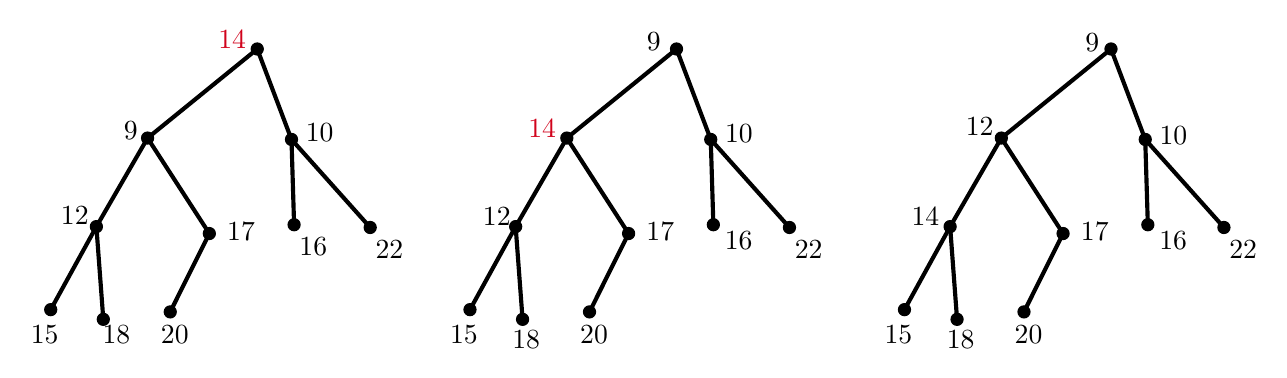
\begin{tikzpicture}[x=0.5pt,y=0.5pt,yscale=-1,xscale=1]
%uncomment if require: \path (0,251); %set diagram left start at 0, and has height of 251

%Flowchart: Connector [id:dp07358279371728427] 
\draw  [fill={rgb, 255:red, 0; green, 0; blue, 0 }  ,fill opacity=1 ] (176.38,20) .. controls (176.38,17.58) and (178.34,15.62) .. (180.75,15.62) .. controls (183.17,15.62) and (185.13,17.58) .. (185.13,20) .. controls (185.13,22.42) and (183.17,24.38) .. (180.75,24.38) .. controls (178.34,24.38) and (176.38,22.42) .. (176.38,20) -- cycle ;
%Flowchart: Connector [id:dp9013708586598245] 
\draw  [fill={rgb, 255:red, 0; green, 0; blue, 0 }  ,fill opacity=1 ] (97.12,84.38) .. controls (97.12,81.96) and (99.08,80) .. (101.5,80) .. controls (103.92,80) and (105.88,81.96) .. (105.88,84.38) .. controls (105.88,86.79) and (103.92,88.75) .. (101.5,88.75) .. controls (99.08,88.75) and (97.12,86.79) .. (97.12,84.38) -- cycle ;
%Flowchart: Connector [id:dp29553697353599095] 
\draw  [fill={rgb, 255:red, 0; green, 0; blue, 0 }  ,fill opacity=1 ] (258,149) .. controls (258,146.58) and (259.96,144.62) .. (262.38,144.62) .. controls (264.79,144.62) and (266.75,146.58) .. (266.75,149) .. controls (266.75,151.42) and (264.79,153.38) .. (262.38,153.38) .. controls (259.96,153.38) and (258,151.42) .. (258,149) -- cycle ;
%Straight Lines [id:da2622599551377074] 
\draw [color={rgb, 255:red, 0; green, 0; blue, 0 }  ,draw opacity=1 ][line width=1.5]    (207.38,147) -- (205.5,85.38) ;
%Straight Lines [id:da633932922371613] 
\draw [color={rgb, 255:red, 0; green, 0; blue, 0 }  ,draw opacity=1 ][line width=1.5]    (101.5,84.38) -- (180.75,20) ;
%Flowchart: Connector [id:dp13162082051454493] 
\draw  [fill={rgb, 255:red, 0; green, 0; blue, 0 }  ,fill opacity=1 ] (201.12,85.38) .. controls (201.12,82.96) and (203.08,81) .. (205.5,81) .. controls (207.92,81) and (209.88,82.96) .. (209.88,85.38) .. controls (209.88,87.79) and (207.92,89.75) .. (205.5,89.75) .. controls (203.08,89.75) and (201.12,87.79) .. (201.12,85.38) -- cycle ;
%Flowchart: Connector [id:dp7155524303373791] 
\draw  [fill={rgb, 255:red, 0; green, 0; blue, 0 }  ,fill opacity=1 ] (60.12,148.38) .. controls (60.12,145.96) and (62.08,144) .. (64.5,144) .. controls (66.92,144) and (68.88,145.96) .. (68.88,148.38) .. controls (68.88,150.79) and (66.92,152.75) .. (64.5,152.75) .. controls (62.08,152.75) and (60.12,150.79) .. (60.12,148.38) -- cycle ;
%Flowchart: Connector [id:dp46343000023437764] 
\draw  [fill={rgb, 255:red, 0; green, 0; blue, 0 }  ,fill opacity=1 ] (27.12,208.38) .. controls (27.12,205.96) and (29.08,204) .. (31.5,204) .. controls (33.92,204) and (35.88,205.96) .. (35.88,208.38) .. controls (35.88,210.79) and (33.92,212.75) .. (31.5,212.75) .. controls (29.08,212.75) and (27.12,210.79) .. (27.12,208.38) -- cycle ;
%Straight Lines [id:da5409521442924461] 
\draw [color={rgb, 255:red, 0; green, 0; blue, 0 }  ,draw opacity=1 ][line width=1.5]    (205.5,85.38) -- (180.75,20) ;
%Straight Lines [id:da6747902580631686] 
\draw [color={rgb, 255:red, 0; green, 0; blue, 0 }  ,draw opacity=1 ][line width=1.5]    (64.5,148.38) -- (101.5,84.38) ;
%Straight Lines [id:da7815420677213977] 
\draw [color={rgb, 255:red, 0; green, 0; blue, 0 }  ,draw opacity=1 ][line width=1.5]    (146.12,153.38) -- (101.5,84.38) ;
%Straight Lines [id:da6594188595232979] 
\draw [color={rgb, 255:red, 0; green, 0; blue, 0 }  ,draw opacity=1 ][line width=1.5]    (31.5,208.38) -- (64.5,148.38) ;
%Flowchart: Connector [id:dp9035939512481367] 
\draw  [fill={rgb, 255:red, 0; green, 0; blue, 0 }  ,fill opacity=1 ] (203,147) .. controls (203,144.58) and (204.96,142.62) .. (207.38,142.62) .. controls (209.79,142.62) and (211.75,144.58) .. (211.75,147) .. controls (211.75,149.42) and (209.79,151.38) .. (207.38,151.38) .. controls (204.96,151.38) and (203,149.42) .. (203,147) -- cycle ;
%Straight Lines [id:da9909770061710292] 
\draw [color={rgb, 255:red, 0; green, 0; blue, 0 }  ,draw opacity=1 ][line width=1.5]    (262.38,149) -- (205.5,85.38) ;
%Flowchart: Connector [id:dp5892893328284525] 
\draw  [fill={rgb, 255:red, 0; green, 0; blue, 0 }  ,fill opacity=1 ] (65.12,215.38) .. controls (65.12,212.96) and (67.08,211) .. (69.5,211) .. controls (71.92,211) and (73.88,212.96) .. (73.88,215.38) .. controls (73.88,217.79) and (71.92,219.75) .. (69.5,219.75) .. controls (67.08,219.75) and (65.12,217.79) .. (65.12,215.38) -- cycle ;
%Flowchart: Connector [id:dp37796994403666173] 
\draw  [fill={rgb, 255:red, 0; green, 0; blue, 0 }  ,fill opacity=1 ] (113.5,210) .. controls (113.5,207.58) and (115.46,205.62) .. (117.88,205.62) .. controls (120.29,205.62) and (122.25,207.58) .. (122.25,210) .. controls (122.25,212.42) and (120.29,214.38) .. (117.88,214.38) .. controls (115.46,214.38) and (113.5,212.42) .. (113.5,210) -- cycle ;
%Flowchart: Connector [id:dp4981451941949617] 
\draw  [fill={rgb, 255:red, 0; green, 0; blue, 0 }  ,fill opacity=1 ] (141.75,153.38) .. controls (141.75,150.96) and (143.71,149) .. (146.12,149) .. controls (148.54,149) and (150.5,150.96) .. (150.5,153.38) .. controls (150.5,155.79) and (148.54,157.75) .. (146.12,157.75) .. controls (143.71,157.75) and (141.75,155.79) .. (141.75,153.38) -- cycle ;
%Straight Lines [id:da07065002309169843] 
\draw [color={rgb, 255:red, 0; green, 0; blue, 0 }  ,draw opacity=1 ][line width=1.5]    (69.5,215.38) -- (64.5,148.38) ;
%Straight Lines [id:da3423526836996703] 
\draw [color={rgb, 255:red, 0; green, 0; blue, 0 }  ,draw opacity=1 ][line width=1.5]    (117.88,210) -- (146.12,153.38) ;
%Flowchart: Connector [id:dp1375963085229701] 
\draw  [fill={rgb, 255:red, 0; green, 0; blue, 0 }  ,fill opacity=1 ] (479.38,20) .. controls (479.38,17.58) and (481.34,15.62) .. (483.75,15.62) .. controls (486.17,15.62) and (488.13,17.58) .. (488.13,20) .. controls (488.13,22.42) and (486.17,24.38) .. (483.75,24.38) .. controls (481.34,24.38) and (479.38,22.42) .. (479.38,20) -- cycle ;
%Flowchart: Connector [id:dp09051194852712707] 
\draw  [fill={rgb, 255:red, 0; green, 0; blue, 0 }  ,fill opacity=1 ] (400.12,84.38) .. controls (400.12,81.96) and (402.08,80) .. (404.5,80) .. controls (406.92,80) and (408.88,81.96) .. (408.88,84.38) .. controls (408.88,86.79) and (406.92,88.75) .. (404.5,88.75) .. controls (402.08,88.75) and (400.12,86.79) .. (400.12,84.38) -- cycle ;
%Flowchart: Connector [id:dp4526533094703221] 
\draw  [fill={rgb, 255:red, 0; green, 0; blue, 0 }  ,fill opacity=1 ] (561,149) .. controls (561,146.58) and (562.96,144.62) .. (565.38,144.62) .. controls (567.79,144.62) and (569.75,146.58) .. (569.75,149) .. controls (569.75,151.42) and (567.79,153.38) .. (565.38,153.38) .. controls (562.96,153.38) and (561,151.42) .. (561,149) -- cycle ;
%Straight Lines [id:da10531615798128313] 
\draw [color={rgb, 255:red, 0; green, 0; blue, 0 }  ,draw opacity=1 ][line width=1.5]    (510.38,147) -- (508.5,85.38) ;
%Straight Lines [id:da09372307643584044] 
\draw [color={rgb, 255:red, 0; green, 0; blue, 0 }  ,draw opacity=1 ][line width=1.5]    (404.5,84.38) -- (483.75,20) ;
%Flowchart: Connector [id:dp8971420943691574] 
\draw  [fill={rgb, 255:red, 0; green, 0; blue, 0 }  ,fill opacity=1 ] (504.12,85.38) .. controls (504.12,82.96) and (506.08,81) .. (508.5,81) .. controls (510.92,81) and (512.88,82.96) .. (512.88,85.38) .. controls (512.88,87.79) and (510.92,89.75) .. (508.5,89.75) .. controls (506.08,89.75) and (504.12,87.79) .. (504.12,85.38) -- cycle ;
%Flowchart: Connector [id:dp12888541856196722] 
\draw  [fill={rgb, 255:red, 0; green, 0; blue, 0 }  ,fill opacity=1 ] (363.12,148.38) .. controls (363.12,145.96) and (365.08,144) .. (367.5,144) .. controls (369.92,144) and (371.88,145.96) .. (371.88,148.38) .. controls (371.88,150.79) and (369.92,152.75) .. (367.5,152.75) .. controls (365.08,152.75) and (363.12,150.79) .. (363.12,148.38) -- cycle ;
%Flowchart: Connector [id:dp37976886359787154] 
\draw  [fill={rgb, 255:red, 0; green, 0; blue, 0 }  ,fill opacity=1 ] (330.12,208.38) .. controls (330.12,205.96) and (332.08,204) .. (334.5,204) .. controls (336.92,204) and (338.88,205.96) .. (338.88,208.38) .. controls (338.88,210.79) and (336.92,212.75) .. (334.5,212.75) .. controls (332.08,212.75) and (330.12,210.79) .. (330.12,208.38) -- cycle ;
%Straight Lines [id:da00382939631379986] 
\draw [color={rgb, 255:red, 0; green, 0; blue, 0 }  ,draw opacity=1 ][line width=1.5]    (508.5,85.38) -- (483.75,20) ;
%Straight Lines [id:da5006261717026612] 
\draw [color={rgb, 255:red, 0; green, 0; blue, 0 }  ,draw opacity=1 ][line width=1.5]    (367.5,148.38) -- (404.5,84.38) ;
%Straight Lines [id:da3231292917624934] 
\draw [color={rgb, 255:red, 0; green, 0; blue, 0 }  ,draw opacity=1 ][line width=1.5]    (449.12,153.38) -- (404.5,84.38) ;
%Straight Lines [id:da6003626275111184] 
\draw [color={rgb, 255:red, 0; green, 0; blue, 0 }  ,draw opacity=1 ][line width=1.5]    (334.5,208.38) -- (367.5,148.38) ;
%Flowchart: Connector [id:dp24928242887719] 
\draw  [fill={rgb, 255:red, 0; green, 0; blue, 0 }  ,fill opacity=1 ] (506,147) .. controls (506,144.58) and (507.96,142.62) .. (510.38,142.62) .. controls (512.79,142.62) and (514.75,144.58) .. (514.75,147) .. controls (514.75,149.42) and (512.79,151.38) .. (510.38,151.38) .. controls (507.96,151.38) and (506,149.42) .. (506,147) -- cycle ;
%Straight Lines [id:da8874329094923221] 
\draw [color={rgb, 255:red, 0; green, 0; blue, 0 }  ,draw opacity=1 ][line width=1.5]    (565.38,149) -- (508.5,85.38) ;
%Flowchart: Connector [id:dp9376179775043852] 
\draw  [fill={rgb, 255:red, 0; green, 0; blue, 0 }  ,fill opacity=1 ] (368.12,215.38) .. controls (368.12,212.96) and (370.08,211) .. (372.5,211) .. controls (374.92,211) and (376.88,212.96) .. (376.88,215.38) .. controls (376.88,217.79) and (374.92,219.75) .. (372.5,219.75) .. controls (370.08,219.75) and (368.12,217.79) .. (368.12,215.38) -- cycle ;
%Flowchart: Connector [id:dp5490426987923039] 
\draw  [fill={rgb, 255:red, 0; green, 0; blue, 0 }  ,fill opacity=1 ] (416.5,210) .. controls (416.5,207.58) and (418.46,205.62) .. (420.88,205.62) .. controls (423.29,205.62) and (425.25,207.58) .. (425.25,210) .. controls (425.25,212.42) and (423.29,214.38) .. (420.88,214.38) .. controls (418.46,214.38) and (416.5,212.42) .. (416.5,210) -- cycle ;
%Flowchart: Connector [id:dp3451316924285829] 
\draw  [fill={rgb, 255:red, 0; green, 0; blue, 0 }  ,fill opacity=1 ] (444.75,153.38) .. controls (444.75,150.96) and (446.71,149) .. (449.12,149) .. controls (451.54,149) and (453.5,150.96) .. (453.5,153.38) .. controls (453.5,155.79) and (451.54,157.75) .. (449.12,157.75) .. controls (446.71,157.75) and (444.75,155.79) .. (444.75,153.38) -- cycle ;
%Straight Lines [id:da35613207019768434] 
\draw [color={rgb, 255:red, 0; green, 0; blue, 0 }  ,draw opacity=1 ][line width=1.5]    (372.5,215.38) -- (367.5,148.38) ;
%Straight Lines [id:da5174013869010234] 
\draw [color={rgb, 255:red, 0; green, 0; blue, 0 }  ,draw opacity=1 ][line width=1.5]    (420.88,210) -- (449.12,153.38) ;
%Flowchart: Connector [id:dp6439356336322] 
\draw  [fill={rgb, 255:red, 0; green, 0; blue, 0 }  ,fill opacity=1 ] (793.38,20) .. controls (793.38,17.58) and (795.34,15.62) .. (797.75,15.62) .. controls (800.17,15.62) and (802.13,17.58) .. (802.13,20) .. controls (802.13,22.42) and (800.17,24.38) .. (797.75,24.38) .. controls (795.34,24.38) and (793.38,22.42) .. (793.38,20) -- cycle ;
%Flowchart: Connector [id:dp21886990424308195] 
\draw  [fill={rgb, 255:red, 0; green, 0; blue, 0 }  ,fill opacity=1 ] (714.12,84.38) .. controls (714.12,81.96) and (716.08,80) .. (718.5,80) .. controls (720.92,80) and (722.88,81.96) .. (722.88,84.38) .. controls (722.88,86.79) and (720.92,88.75) .. (718.5,88.75) .. controls (716.08,88.75) and (714.12,86.79) .. (714.12,84.38) -- cycle ;
%Flowchart: Connector [id:dp03837895619274634] 
\draw  [fill={rgb, 255:red, 0; green, 0; blue, 0 }  ,fill opacity=1 ] (875,149) .. controls (875,146.58) and (876.96,144.62) .. (879.38,144.62) .. controls (881.79,144.62) and (883.75,146.58) .. (883.75,149) .. controls (883.75,151.42) and (881.79,153.38) .. (879.38,153.38) .. controls (876.96,153.38) and (875,151.42) .. (875,149) -- cycle ;
%Straight Lines [id:da14782465407982648] 
\draw [color={rgb, 255:red, 0; green, 0; blue, 0 }  ,draw opacity=1 ][line width=1.5]    (824.38,147) -- (822.5,85.38) ;
%Straight Lines [id:da008115829235638361] 
\draw [color={rgb, 255:red, 0; green, 0; blue, 0 }  ,draw opacity=1 ][line width=1.5]    (718.5,84.38) -- (797.75,20) ;
%Flowchart: Connector [id:dp749580488735119] 
\draw  [fill={rgb, 255:red, 0; green, 0; blue, 0 }  ,fill opacity=1 ] (818.12,85.38) .. controls (818.12,82.96) and (820.08,81) .. (822.5,81) .. controls (824.92,81) and (826.88,82.96) .. (826.88,85.38) .. controls (826.88,87.79) and (824.92,89.75) .. (822.5,89.75) .. controls (820.08,89.75) and (818.12,87.79) .. (818.12,85.38) -- cycle ;
%Flowchart: Connector [id:dp721237398452121] 
\draw  [fill={rgb, 255:red, 0; green, 0; blue, 0 }  ,fill opacity=1 ] (677.12,148.38) .. controls (677.12,145.96) and (679.08,144) .. (681.5,144) .. controls (683.92,144) and (685.88,145.96) .. (685.88,148.38) .. controls (685.88,150.79) and (683.92,152.75) .. (681.5,152.75) .. controls (679.08,152.75) and (677.12,150.79) .. (677.12,148.38) -- cycle ;
%Flowchart: Connector [id:dp8969752490868951] 
\draw  [fill={rgb, 255:red, 0; green, 0; blue, 0 }  ,fill opacity=1 ] (644.12,208.38) .. controls (644.12,205.96) and (646.08,204) .. (648.5,204) .. controls (650.92,204) and (652.88,205.96) .. (652.88,208.38) .. controls (652.88,210.79) and (650.92,212.75) .. (648.5,212.75) .. controls (646.08,212.75) and (644.12,210.79) .. (644.12,208.38) -- cycle ;
%Straight Lines [id:da1950712786856147] 
\draw [color={rgb, 255:red, 0; green, 0; blue, 0 }  ,draw opacity=1 ][line width=1.5]    (822.5,85.38) -- (797.75,20) ;
%Straight Lines [id:da5410491903490715] 
\draw [color={rgb, 255:red, 0; green, 0; blue, 0 }  ,draw opacity=1 ][line width=1.5]    (681.5,148.38) -- (718.5,84.38) ;
%Straight Lines [id:da13743949368590924] 
\draw [color={rgb, 255:red, 0; green, 0; blue, 0 }  ,draw opacity=1 ][line width=1.5]    (763.12,153.38) -- (718.5,84.38) ;
%Straight Lines [id:da3696523456420949] 
\draw [color={rgb, 255:red, 0; green, 0; blue, 0 }  ,draw opacity=1 ][line width=1.5]    (648.5,208.38) -- (681.5,148.38) ;
%Flowchart: Connector [id:dp0084873615551605] 
\draw  [fill={rgb, 255:red, 0; green, 0; blue, 0 }  ,fill opacity=1 ] (820,147) .. controls (820,144.58) and (821.96,142.62) .. (824.38,142.62) .. controls (826.79,142.62) and (828.75,144.58) .. (828.75,147) .. controls (828.75,149.42) and (826.79,151.38) .. (824.38,151.38) .. controls (821.96,151.38) and (820,149.42) .. (820,147) -- cycle ;
%Straight Lines [id:da27565732300312706] 
\draw [color={rgb, 255:red, 0; green, 0; blue, 0 }  ,draw opacity=1 ][line width=1.5]    (879.38,149) -- (822.5,85.38) ;
%Flowchart: Connector [id:dp5637778962512422] 
\draw  [fill={rgb, 255:red, 0; green, 0; blue, 0 }  ,fill opacity=1 ] (682.12,215.38) .. controls (682.12,212.96) and (684.08,211) .. (686.5,211) .. controls (688.92,211) and (690.88,212.96) .. (690.88,215.38) .. controls (690.88,217.79) and (688.92,219.75) .. (686.5,219.75) .. controls (684.08,219.75) and (682.12,217.79) .. (682.12,215.38) -- cycle ;
%Flowchart: Connector [id:dp06500857183698838] 
\draw  [fill={rgb, 255:red, 0; green, 0; blue, 0 }  ,fill opacity=1 ] (730.5,210) .. controls (730.5,207.58) and (732.46,205.62) .. (734.88,205.62) .. controls (737.29,205.62) and (739.25,207.58) .. (739.25,210) .. controls (739.25,212.42) and (737.29,214.38) .. (734.88,214.38) .. controls (732.46,214.38) and (730.5,212.42) .. (730.5,210) -- cycle ;
%Flowchart: Connector [id:dp13396637654961707] 
\draw  [fill={rgb, 255:red, 0; green, 0; blue, 0 }  ,fill opacity=1 ] (758.75,153.38) .. controls (758.75,150.96) and (760.71,149) .. (763.12,149) .. controls (765.54,149) and (767.5,150.96) .. (767.5,153.38) .. controls (767.5,155.79) and (765.54,157.75) .. (763.12,157.75) .. controls (760.71,157.75) and (758.75,155.79) .. (758.75,153.38) -- cycle ;
%Straight Lines [id:da03208959858971949] 
\draw [color={rgb, 255:red, 0; green, 0; blue, 0 }  ,draw opacity=1 ][line width=1.5]    (686.5,215.38) -- (681.5,148.38) ;
%Straight Lines [id:da9350323425263134] 
\draw [color={rgb, 255:red, 0; green, 0; blue, 0 }  ,draw opacity=1 ][line width=1.5]    (734.88,210) -- (763.12,153.38) ;

% Text Node
\draw (15.24,218.06) node [anchor=north west][inner sep=0.75pt]   [align=left] {$\displaystyle 15$};
% Text Node
\draw (82.38,70.38) node [anchor=north west][inner sep=0.75pt]   [align=left] {$\displaystyle 9$};
% Text Node
\draw (264.38,156.38) node [anchor=north west][inner sep=0.75pt]   [align=left] {$\displaystyle 22$};
% Text Node
\draw (150.75,5) node [anchor=north west][inner sep=0.75pt]   [align=left] {$\displaystyle \textcolor[rgb]{0.82,0.01,0.11}{14}$};
% Text Node
\draw (36.97,131.91) node [anchor=north west][inner sep=0.75pt]   [align=left] {$\displaystyle 12$};
% Text Node
\draw (213.97,71.91) node [anchor=north west][inner sep=0.75pt]   [align=left] {$\displaystyle 10$};
% Text Node
\draw (209.38,154.38) node [anchor=north west][inner sep=0.75pt]   [align=left] {$\displaystyle 16$};
% Text Node
\draw (67.12,218.38) node [anchor=north west][inner sep=0.75pt]   [align=left] {$\displaystyle 18$};
% Text Node
\draw (109.25,218) node [anchor=north west][inner sep=0.75pt]   [align=left] {$\displaystyle 20$};
% Text Node
\draw (157.12,143.75) node [anchor=north west][inner sep=0.75pt]   [align=left] {$\displaystyle 17$};
% Text Node
\draw (318.24,218.06) node [anchor=north west][inner sep=0.75pt]   [align=left] {$\displaystyle 15$};
% Text Node
\draw (567.38,156.38) node [anchor=north west][inner sep=0.75pt]   [align=left] {$\displaystyle 22$};
% Text Node
\draw (516.75,150) node [anchor=north west][inner sep=0.75pt]   [align=left] {$\displaystyle 16$};
% Text Node
\draw (516.97,72.91) node [anchor=north west][inner sep=0.75pt]   [align=left] {$\displaystyle 10$};
% Text Node
\draw (363.24,221.47) node [anchor=north west][inner sep=0.75pt]   [align=left] {$\displaystyle 18$};
% Text Node
\draw (412.25,218) node [anchor=north west][inner sep=0.75pt]   [align=left] {$\displaystyle 20$};
% Text Node
\draw (460.12,143.75) node [anchor=north west][inner sep=0.75pt]   [align=left] {$\displaystyle 17$};
% Text Node
\draw (632.24,218.06) node [anchor=north west][inner sep=0.75pt]   [align=left] {$\displaystyle 15$};
% Text Node
\draw (777.38,7.38) node [anchor=north west][inner sep=0.75pt]   [align=left] {$\displaystyle 9$};
% Text Node
\draw (881.38,156.38) node [anchor=north west][inner sep=0.75pt]   [align=left] {$\displaystyle 22$};
% Text Node
\draw (830.75,150) node [anchor=north west][inner sep=0.75pt]   [align=left] {$\displaystyle 16$};
% Text Node
\draw (830.97,73.91) node [anchor=north west][inner sep=0.75pt]   [align=left] {$\displaystyle 10$};
% Text Node
\draw (677.24,221.47) node [anchor=north west][inner sep=0.75pt]   [align=left] {$\displaystyle 18$};
% Text Node
\draw (726.25,218) node [anchor=north west][inner sep=0.75pt]   [align=left] {$\displaystyle 20$};
% Text Node
\draw (774.12,143.75) node [anchor=north west][inner sep=0.75pt]   [align=left] {$\displaystyle 17$};
% Text Node
\draw (460.38,6.38) node [anchor=north west][inner sep=0.75pt]   [align=left] {$\displaystyle 9$};
% Text Node
\draw (374.75,69) node [anchor=north west][inner sep=0.75pt]   [align=left] {$\displaystyle \textcolor[rgb]{0.82,0.01,0.11}{14}$};
% Text Node
\draw (341.97,132.91) node [anchor=north west][inner sep=0.75pt]   [align=left] {$\displaystyle 12$};
% Text Node
\draw (651.75,133) node [anchor=north west][inner sep=0.75pt]   [align=left] {$\displaystyle \textcolor[rgb]{0,0,0}{14}$};
% Text Node
\draw (690.97,67.91) node [anchor=north west][inner sep=0.75pt]   [align=left] {$\displaystyle 12$};


\end{tikzpicture}

}
\caption{Illustrating sift-down procedure.}
\end{figure}

We finally give the pseudo-code for implementing the binary heap.
We not only maintain the array $S$ but also the number of elements in $S$, denoted as $n$.

\begin{minipage}{0.8\textwidth}
	\aaA {3}{function empty($PQ$)}\xxx
	\aab {if $n = 0$: return true;}\xxx
	\aab {else: return true;}\xxx
	\aaa {end function;}\xxx
\end{minipage}

\begin{minipage}{0.8\textwidth}
	\aaA {4}{function insert($PQ$, $x$)}\xxx
	\aab {$n = n + 1$;}\xxx
	\aab {$S[n] = x$;}\xxx
	\aab {bubble-up~($S$, $n$);}\xxx
	\aaa {end function;}\xxx
\end{minipage}

\begin{minipage}{0.8\textwidth}
	\aaA {2}{function find-min($PQ$)}\xxx
	\aab {return $S[1]$;}\xxx
	\aaa {end function;}\xxx
\end{minipage}

\begin{minipage}{0.8\textwidth}
	\aaA {4}{function delete-min($PQ$)}\xxx
	\aab {$S[1] = S[n]$;}\xxx
	\aab {$n = n - 1$;}\xxx
	\aab {sift-down~($S$, $1$);}\xxx
	\aaa {end function;}\xxx
\end{minipage}

\begin{minipage}{0.8\textwidth}
	\aaA {3}{function decrease-key($PQ$, $k$, new-key)}\xxx
	\aab {$S[k].key = $ new-key;}\xxx
	\aab {bubble-up~($S$, $k$);}\xxx
	\aaa {end function;}\xxx
\end{minipage}

Both bubble-up and sift-down procedures runs in $O(\log n)$ time.
This is because, a complete binary tree with $n$ vertices has a height of $\log n$, while
the worst case of either procedure traverses along a path between the root and a leaf.
Formally, in each recursive call, $k$ is either halved or doubled, and hence the number
of recursive calls is $\log n$.
The empty and find-min procedures takes $\Theta(1)$ time; the other 3 procedures takes $O(\log n)$ time, as they are dominated by either bubble-up or sift-down.


